\documentclass[journal]{IEEEtran}

\usepackage{amsmath,amssymb,amsfonts}
\usepackage{amsthm}
\usepackage{graphicx}
\usepackage{booktabs}
\usepackage{multirow}
\usepackage{algorithm}
\usepackage{algorithmic}
\usepackage{cite}
\usepackage{url}
\usepackage[hidelinks]{hyperref}

\setlength{\textfloatsep}{8pt plus 2pt minus 2pt}
\setlength{\floatsep}{8pt plus 2pt minus 2pt}
\setlength{\dbltextfloatsep}{8pt plus 2pt minus 2pt}
\setlength{\dblfloatsep}{8pt plus 2pt minus 2pt}
\setlength{\abovecaptionskip}{3pt}
\setlength{\belowcaptionskip}{0pt}
\makeatletter
\setlength{\@fptop}{0pt}
\setlength{\@fpsep}{8pt plus 2pt minus 2pt}
\setlength{\@fpbot}{0pt plus 1fil}
\setlength{\@dblfptop}{0pt}
\setlength{\@dblfpsep}{8pt plus 2pt minus 2pt}
\setlength{\@dblfpbot}{0pt plus 1fil}
\makeatother

% Shared notation for the TAC manuscript.
\newcommand{\R}{\mathbb{R}}
\newcommand{\N}{\mathbb{N}}
\newcommand{\Tset}{\mathcal{T}}
\newcommand{\Rset}{\mathcal{R}}
\newcommand{\Pset}{\mathcal{P}}
\newcommand{\Sset}{\mathcal{S}}
\newcommand{\Cset}{\mathcal{C}}
\newcommand{\Oset}{\mathcal{O}}
\newcommand{\Ggraph}{\mathcal{G}}
\newcommand{\cost}{\operatorname{cost}}
\newcommand{\dist}{\operatorname{dist}}
\newcommand{\argmin}{\operatorname*{arg\,min}}
\newcommand{\argmax}{\operatorname*{arg\,max}}
\newcommand{\reachable}{\operatorname{reach}}
\newcommand{\cover}{\operatorname{cov}}
\newcommand{\safe}{\operatorname{safe}}
\newcommand{\heading}{\operatorname{head}}
\newcommand{\approach}{\operatorname{app}}
\newcommand{\length}{\operatorname{len}}
\newcommand{\uncovered}{\operatorname{uncov}}


\newtheorem{definition}{Definition}
\newtheorem{assumption}{Assumption}
\newtheorem{proposition}{Proposition}
\newtheorem{remark}{Remark}

\title{A Constrained Hierarchical Planning Framework for Reachability-Aware Multi-Task Mobile Manipulation}

\author{
Peng Dai
\thanks{Peng Dai is with the School of Automation,
Xi'an University of Posts and Telecommunications,
Xi'an, China.
E-mail: xxx@xxx.com.}
}

\begin{document}

\maketitle
\raggedbottom

\begin{abstract}
Multi-table mobile manipulation requires a robot to decide not only how to move between workspaces, but also where to dock so that tabletop tasks are reachable by its manipulators. Treating tabletop task points as navigation goals ignores the mismatch between the mobile-base configuration space and the arm workspace, and can produce short paths that leave manipulation tasks infeasible. This paper presents RCH-MT-MMP, a reachability-constrained hierarchical planning framework for multi-task dual-arm mobile manipulation. The framework partitions tabletop tasks into local task regions, generates collision-free candidate docking poses around each table, evaluates each pose using task coverage, dual-arm reachability, safety distance, orientation consistency, and approach cost, and then selects one or more docking poses per table through a coverage-aware greedy strategy. The selected docking poses are finally connected by a replaceable global path planner. A feasibility result shows that the multi-docking selection terminates with full task coverage whenever each task is covered by at least one feasible candidate. Experiments on a 16-table scenario complete 36/36 tasks with 27 docking poses and a 63.29 m route. Across submission-level baselines, the full method preserves 100.00\% completion, whereas single-docking and nearest-docking variants achieve 73.73\% and 25.59\% mean completion, respectively. These results indicate that reachability-aware docking decisions should precede global path shortening in mobile manipulation planning.

\end{abstract}

\begin{IEEEkeywords}
Mobile manipulation, hierarchical planning, reachability constraints, set cover, docking pose selection, path planning.
\end{IEEEkeywords}

\section{Introduction}
\label{sec:introduction}

Mobile dual-arm robots are increasingly expected to service multiple workspaces in laboratories, restaurants, warehouses, and human-assistance environments. Recent studies on mobile manipulation and task-and-motion planning show that such robots must coordinate navigation, base placement, arm feasibility, and task execution rather than solve them as isolated modules \cite{sandakalum2022motion,zhao2024survey,zhang2022grop,gu2023multiskill,fu2024mobilealoha}. In multi-table service settings, the robot must navigate between tables or benches while executing manipulation tasks distributed over tabletop surfaces. The central planning question is therefore not only how to find a collision-free base path, but also how to choose base poses from which the arms can actually reach the assigned objects or task points.

The difficulty arises because tabletop task coordinates are not valid navigation goals for the mobile base. A task point may be inside the arm workspace from one side of a table but unreachable from another side, while the mobile base must remain outside the table footprint and satisfy clearance and orientation constraints. A planner that directly connects task locations in the ground plane can report a short path even when no feasible arm motion exists after arrival. This mismatch is especially severe for dual-arm platforms, where left-arm and right-arm reachability, table geometry, and approach direction jointly determine whether a docking pose is useful.

Existing motion-planning methods solve important parts of the problem but do not fully address this decision layer. Grid and graph search methods such as Dijkstra's algorithm and A* provide reliable global path planning in known maps \cite{dijkstra1959note,hart1968formal,liu2023pathplanning}, and any-angle or symmetry-reduced variants can reduce path length or search effort \cite{nash2007theta,harabor2011online}. Mobile-manipulation studies have examined robot placement, reachability priors, approach uncertainty, and base-pose sequence planning \cite{reister2022combining,jauhri2022reachability,yamazaki2022approaching,naik2024basenet}. However, tightly coupled planning over all base, arm, and task-order variables remains costly for multi-table scenes. Coverage and viewpoint-selection methods reason about covering spatial targets, yet they often lack explicit dual-arm reachability constraints and route-level integration.

The first limitation is that path optimality can conflict with manipulation feasibility. A nearest docking or shortest-route choice may reduce travel distance while leaving many tabletop tasks uncovered. The experiments in this paper show this failure mode directly: nearest docking achieves only 50.00\% completion in the main scenario and drops to 0.00\% in hard mixed task distributions. Thus, for mobile manipulation, coverage and reachability should be treated as feasibility conditions before route length is minimized.

The second limitation is that a single docking pose is often insufficient for a complex table. Tasks can lie on different sides or near reachability boundaries, and no single base pose may cover all of them. Enforcing one docking pose per table converts a physically feasible multi-stop operation into an infeasible planning problem. A planner therefore needs a mechanism that allows multiple docking poses to jointly cover the same tabletop region.

The third limitation is that global path planning and docking selection are often evaluated separately. A mobile-manipulation planner should preserve a clean interface between local manipulation feasibility and global navigation so that different global planners can be benchmarked under the same selected docking set. This modularity is important for reproducibility, algorithm comparison, and deployment in different map or robot settings.

Based on these observations, this paper proposes RCH-MT-MMP, a reachability-constrained hierarchical planning framework that transforms tabletop tasks into reachable docking-pose coverage decisions and then connects the selected docking poses through a constrained global routing layer.

The contributions are as follows.

\begin{enumerate}
    \item A constrained hierarchical formulation is introduced for multi-table dual-arm mobile manipulation. The formulation separates local docking feasibility from global route connection while keeping them in a single objective that penalizes uncovered tasks, docking cost, and route length.
    \item A candidate docking-pose evaluation method is developed using task coverage, dual-arm reachability, safety distance, orientation consistency, and approach cost. This scoring rule converts geometric task distributions into ranked service poses suitable for dual-arm operation.
    \item A coverage-aware multi-docking selection strategy is designed so that one table may be covered by several docking poses. Under a mild candidate-coverage condition, the greedy selection loop terminates with full coverage in finite time.
    \item A unified experimental pipeline is provided for main scenes, hard task distributions, ablations, random-scale studies, noise and stress tests, small-scale oracle references, and global-planner benchmarks. In submission-level experiments, the full method maintains 100.00\% completion, while single-docking and nearest-docking baselines leave substantial tasks uncovered.
\end{enumerate}

The rest of the paper is organized as follows. Section~\ref{sec:related} reviews related work. Section~\ref{sec:problem} formulates the constrained docking and routing problem. Section~\ref{sec:method} presents the proposed framework. Section~\ref{sec:analysis} gives feasibility and complexity analysis. Section~\ref{sec:experiments} reports the experimental evidence, and Section~\ref{sec:conclusion} concludes the paper.

\section{Related Work}
\label{sec:related}

\subsection{Global Path Planning}
Classical graph-search algorithms provide the routing foundation for many mobile-robot systems. Dijkstra's algorithm gives shortest paths on graphs with nonnegative edge weights \cite{dijkstra1959note}, while A* accelerates search by adding an admissible heuristic \cite{hart1968formal}. For grid maps, variants such as Jump Point Search exploit path symmetries \cite{harabor2011online}, and Theta* relaxes grid-constrained headings to produce any-angle paths \cite{nash2007theta}. Recent surveys continue to emphasize that path planning must balance optimality, efficiency, map representation, and robustness in mobile-robot applications \cite{liu2023pathplanning}. These methods are effective for connecting navigation states, but they do not decide which navigation states should be visited for manipulation. This paper therefore treats global planners as replaceable routing modules after reachability-aware docking poses have been selected.

\subsection{Mobile Manipulation and Base Placement}
Mobile manipulation planning combines base motion with arm feasibility, grasping, and task execution \cite{siciliano2009robotics,lynch2017modern}. Recent reviews and task-and-motion planning studies further show that mobile manipulation requires coordination between symbolic task decisions, robot placement, perception, and continuous motion feasibility \cite{sandakalum2022motion,zhao2024survey,zhang2022grop}. Learning-based systems and benchmarks have extended this setting to object rearrangement, bimanual mobile manipulation, last-mile navigation, and tabletop rearrangement \cite{gu2023multiskill,fu2024mobilealoha,zhang2025momakitchen,hu2025mobiletabletop}. These works motivate the need to reason about where the mobile base should stand before manipulation is attempted. The present paper focuses on a complementary geometric planning layer: given tabletop task points and known scene geometry, it selects one or more reachable docking poses per table and then connects them with a global route.

\subsection{Reachability-Aware Docking and Base-Pose Selection}
A common strategy in mobile manipulation is to sample feasible base placements and evaluate manipulation reachability or inverse-kinematic feasibility. Recent work has combined navigation and manipulation costs for robot placement \cite{reister2022combining}, learned reachability behavior priors \cite{jauhri2022reachability}, considered approach planning under pose uncertainty \cite{yamazaki2022approaching}, optimized base placement for coverage mobile manipulation \cite{zhang2023baseplacement}, and used manipulability or dexterity maps to characterize useful arm workspaces \cite{sereinig2024comfort,yao2024edm}. Base-pose sequence planning has also been studied for pickup tasks \cite{naik2024basenet}. These studies are closely related to the docking-pose candidates used here. The difference is that the present problem involves many tabletop task points across many tables, so a base placement is valuable only through the subset of tasks it covers and through its effect on the global route. The proposed framework therefore treats base placement as a constrained coverage decision rather than an isolated local feasibility test.

\subsection{Coverage, Viewpoint, and Service-Pose Selection}
Coverage planning studies how a robot can visit or observe regions of interest \cite{choset2001coverage}. Viewpoint planning and frontier-based exploration similarly select poses that cover sensing targets or unknown space \cite{yamauchi1997frontier}. These problems share a set-cover structure with docking-pose selection: each candidate pose covers a subset of targets, and the planner must choose a useful subset. However, tabletop manipulation differs from sensing coverage because coverage depends on dual-arm reachability, table-side geometry, safety clearance, and docking orientation. The candidate score in this paper augments coverage with these manipulation-specific constraints.

\subsection{Hierarchical and Constraint-Based Planning}
Hierarchical planning reduces a large coupled planning problem into structured subproblems. In mobile manipulation, this separation is attractive because full joint optimization over task assignment, base route, and arm motion can be computationally expensive \cite{zhao2024survey}. Set cover and greedy selection provide practical approximations for selecting service poses \cite{chvatal1979greedy}, while routing heuristics are often used after goal states are chosen \cite{lavalle2006planning}. The proposed framework follows this hierarchical philosophy but makes the interface explicit: local candidates expose coverage and reachability sets, and the global layer only routes selected docking poses. This separation enables the same docking decisions to be tested with A*, Dijkstra, JPS, GBFS, Theta*, Lazy Theta*, and Convex A* planners in the experiments.

\section{Problem Formulation}
\label{sec:problem}

\subsection{Environment and Tasks}
Consider a known planar workspace represented by an occupancy grid
\(\Ggraph=(V,E)\), where occupied cells correspond to walls, tables, or other obstacles. Let
\(\Rset=\{R_j\}_{j=1}^{M}\) denote the set of tabletop task regions and
\(\Tset=\{t_i\}_{i=1}^{N}\) denote all tabletop task points. Each task \(t_i\) lies on one table region and requires a mobile dual-arm robot to dock near the table before executing a manipulation primitive.

A docking pose is denoted by \(p=(x,y,\theta)\), where \((x,y)\) is the base position in the ground plane and \(\theta\) is the base heading. For each table \(R_j\), a finite set of candidate docking poses \(\Pset_j=\{p_{jk}\}_{k=1}^{K_j}\) is sampled around feasible table sides. The complete candidate set is \(\Pset=\cup_j \Pset_j\).

\subsection{Reachability and Coverage}
The reachability score between a docking pose \(p\) and a task \(t\) is written as \(\rho(p,t)\in[0,1]\). It summarizes geometric arm reachability, side consistency, and distance from the arm workspace boundary. A task is covered by a docking pose if the score exceeds a threshold and the pose satisfies safety and collision constraints:
\begin{equation}
    t \in C(p)
    \quad \Longleftrightarrow \quad
    \rho(p,t) \geq \rho_{\min}, \quad \safe(p)=1 .
    \label{eq:coverage}
\end{equation}
The set \(C(p)\subseteq\Tset\) is the task coverage set of pose \(p\). For a selected docking set \(\Sset\subseteq\Pset\), the uncovered task set is
\begin{equation}
    U(\Sset)=\Tset \setminus \bigcup_{p\in\Sset} C(p).
    \label{eq:uncovered}
\end{equation}

\subsection{Candidate Cost}
Each candidate is assigned a local cost
\begin{equation}
    J(p)=w_c J_c(p)+w_r J_r(p)+w_s J_s(p)+w_h J_h(p)+w_a J_a(p),
    \label{eq:local_cost}
\end{equation}
where \(J_c\) penalizes weak task coverage, \(J_r\) penalizes low average reachability, \(J_s\) penalizes unsafe clearance, \(J_h\) penalizes poor docking orientation, and \(J_a\) penalizes approach cost from the surrounding free space. Lower \(J(p)\) indicates a more useful local docking pose.

\subsection{Hierarchical Objective}
The planning problem is to select a docking subset \(\Sset\) and a visit order over that subset. Let \(L(\Sset)\) denote the length of the global route that starts from the robot initial pose, visits the selected docking poses, and returns if required. The hierarchical objective is
\begin{equation}
\min_{\Sset\subseteq\Pset}
    \lambda_1 |U(\Sset)|
    + \lambda_2 \sum_{p\in\Sset} J(p)
    + \lambda_3 L(\Sset).
\label{eq:objective}
\end{equation}
The weight \(\lambda_1\) is chosen to prioritize task completion over path shortening. This reflects the physical requirement that a short route is not useful if the robot cannot manipulate the assigned tabletop tasks after arriving.

\begin{remark}
Equation~\eqref{eq:objective} has a set-cover component and a routing component. The resulting problem is combinatorial even after discretizing candidate docking poses. The proposed method therefore solves it hierarchically: it first greedily selects coverage-effective docking poses and then routes the selected poses with a global planner.
\end{remark}

\section{Proposed Method}
\label{sec:method}

\subsection{Framework Overview}
RCH-MT-MMP converts a multi-table manipulation problem into two coupled but modular layers. The local layer generates and scores candidate docking poses around each table. The selection layer chooses one or more poses per table to cover the remaining tasks. The global layer connects the selected docking poses in the occupancy grid. This design keeps the manipulation feasibility decision visible before the path planner optimizes travel.

\subsection{Task Region Partition}
Tasks are first assigned to tabletop regions according to the table polygons or bounding boxes. This partition restricts candidate generation to the local geometry of each table and avoids comparing candidates that serve unrelated regions. For table \(R_j\), the task subset is \(\Tset_j=\{t_i:t_i\in R_j\}\), and \(\Tset=\cup_j \Tset_j\).

\subsection{Candidate Generation and Evaluation}
Candidate docking poses are sampled along feasible table sides with headings oriented toward the table. Candidates that collide with obstacles or violate the required safety distance are removed. For each remaining candidate, the planner computes the coverage set \(C(p)\), average reachability over covered tasks, orientation consistency, and approach cost. Algorithm~\ref{alg:candidate} summarizes this stage.

\begin{algorithm}[t]
\caption{Candidate docking-pose generation and evaluation}
\label{alg:candidate}
\begin{algorithmic}[1]
\REQUIRE Table regions \(\Rset\), tasks \(\Tset\), occupancy grid \(\Ggraph\)
\ENSURE Candidate set \(\Pset\) with coverage sets and costs
\STATE \(\Pset \leftarrow \emptyset\)
\FOR{each table \(R_j\in\Rset\)}
    \STATE Generate side-aligned docking samples \(\Pset_j\)
    \FOR{each \(p\in\Pset_j\)}
        \IF{\(\safe(p)=0\) or \(p\) is in collision}
            \STATE discard \(p\)
        \ELSE
            \STATE Compute \(\rho(p,t)\) for all \(t\in\Tset_j\)
            \STATE Build \(C(p)\) using \eqref{eq:coverage}
            \STATE Compute \(J(p)\) using \eqref{eq:local_cost}
            \STATE \(\Pset \leftarrow \Pset \cup \{p\}\)
        \ENDIF
    \ENDFOR
\ENDFOR
\RETURN \(\Pset\)
\end{algorithmic}
\end{algorithm}

\subsection{Coverage-Aware Multi-Docking Selection}
For each table, the planner maintains a set of remaining uncovered tasks. At each iteration, it selects the candidate that provides the best tradeoff between newly covered tasks and local cost. Unlike single-docking strategies, the loop is allowed to select multiple candidates for the same table until all tasks are covered or no useful candidate remains. Algorithm~\ref{alg:selection} gives the complete selection and routing interface.

\begin{algorithm}[t]
\caption{Multi-docking selection and global routing}
\label{alg:selection}
\begin{algorithmic}[1]
\REQUIRE Candidate set \(\Pset\), tasks \(\Tset\), global planner \(\Pi\)
\ENSURE Selected docking set \(\Sset\), route \(\Gamma\)
\STATE \(\Sset\leftarrow\emptyset\), \(U\leftarrow\Tset\)
\WHILE{\(U\neq\emptyset\)}
    \STATE \(p^\star \leftarrow \argmin_{p\in\Pset} \frac{J(p)}{|C(p)\cap U|+\epsilon}\)
    \IF{\(C(p^\star)\cap U=\emptyset\)}
        \STATE break
    \ENDIF
    \STATE \(\Sset\leftarrow\Sset\cup\{p^\star\}\)
    \STATE \(U\leftarrow U\setminus C(p^\star)\)
    \STATE Remove \(p^\star\) from \(\Pset\)
\ENDWHILE
\STATE Compute pairwise path costs between poses in \(\Sset\) using \(\Pi\)
\STATE Select a visit order with a routing heuristic
\STATE Stitch pairwise paths into global route \(\Gamma\)
\RETURN \(\Sset,\Gamma\)
\end{algorithmic}
\end{algorithm}

\subsection{Global Docking-Pose Routing}
After docking selection, global routing is performed over the selected docking set rather than over the original tabletop task points. A planner \(\Pi\) computes collision-free paths between docking poses. The implementation supports A*, Dijkstra, JPS, GBFS, Theta*, Lazy Theta*, and Convex A*, which allows the routing layer to be benchmarked without changing the docking selection logic. The default route order is computed using a greedy nearest-neighbor heuristic over the pairwise path-cost matrix.

\section{Feasibility and Complexity Analysis}
\label{sec:analysis}

\begin{assumption}[Candidate coverage]
\label{ass:coverage}
For every task \(t_i\in\Tset\), there exists at least one collision-free candidate docking pose \(p\in\Pset\) such that \(t_i\in C(p)\).
\end{assumption}

\begin{proposition}[Finite full-coverage selection]
\label{prop:coverage}
Under Assumption~\ref{ass:coverage}, if the selection loop always chooses a candidate that covers at least one remaining uncovered task whenever such a candidate exists, then the multi-docking selection terminates in at most \(N\) successful iterations with \(U(\Sset)=\emptyset\).
\end{proposition}

\begin{proof}
At the start of the selection loop, \(U=\Tset\). At any successful iteration, the selected candidate \(p^\star\) satisfies \(C(p^\star)\cap U\neq\emptyset\), so at least one task is removed from \(U\). Since \(U\) contains at most \(N\) tasks and no removed task is reinserted, there can be at most \(N\) successful iterations. Assumption~\ref{ass:coverage} guarantees that, while \(U\neq\emptyset\), at least one feasible candidate exists for each remaining task. Therefore the loop cannot stop due to lack of coverage before all tasks are removed, and it terminates with \(U(\Sset)=\emptyset\).
\end{proof}

\begin{proposition}[Computational complexity]
\label{prop:complexity}
Let \(K=|\Pset|\), \(N=|\Tset|\), \(Q=|\Sset|\), and let \(C_{\Pi}\) denote the cost of one global path-planner query. Candidate evaluation has worst-case complexity \(O(KN)\). Greedy multi-docking selection has worst-case complexity \(O(KN)\) when coverage intersections are updated explicitly. Pairwise global path-cost computation has complexity \(O(Q^2 C_{\Pi})\), and greedy route ordering has complexity \(O(Q^2)\).
\end{proposition}

\begin{proof}
Each candidate may be evaluated against every task in the worst case, giving \(O(KN)\). During selection, each candidate-task coverage relation can be inspected while computing newly covered tasks; explicit updates therefore give \(O(KN)\) over the loop. The route layer queries the global planner for each ordered or unordered pair of selected docking poses, which is \(O(Q^2)\) calls up to a constant factor. The nearest-neighbor route heuristic repeatedly scans remaining docking poses, giving \(O(Q^2)\).
\end{proof}

\begin{remark}[Approximation scope]
The docking selection resembles weighted set cover, and the route layer resembles a traveling-salesman routing problem over selected docking poses. The present paper does not claim global optimality for \eqref{eq:objective}. Instead, it provides a finite-termination feasibility condition, complexity characterization, and small-scale oracle-reference experiments that estimate the practical gap within bounded candidate sets.
\end{remark}

\section{Experiments}
\label{sec:experiments}

\subsection{Experimental Setup}
The experiments use the current MATLAB implementation of the RCH-MT-MMP pipeline.
 The main benchmark is a \(10\,\mathrm{m}\times 10\,\mathrm{m}\) indoor 
 tabletop-service scene with 16 rectangular tables arranged in four rows and 36 tabletop task points distributed 
 over the table surfaces. This setting tests the decision layer that precedes arm execution: 
 the robot must determine which collision-free docking poses make the tabletop tasks reachable, 
 select enough poses to cover all tasks, and connect the selected poses with a global route.

Figure~\ref{fig:main_scenario_scene} shows the main scene and the resulting plan.
 Gray rectangles denote tables, green circles denote tabletop task points, 
 orange triangles denote selected docking poses, the blue polyline denotes the global navigation path, 
 and the red star denotes the start state. Several tables require more than one docking pose because task points on different sides
  cannot all be reached from a single base placement under the dual-arm reachability and clearance constraints. 
  The default global planner is A*, and all reported submission-level data are generated from the `submission' experiment mode.

\begin{figure}[!t]
    \centering
    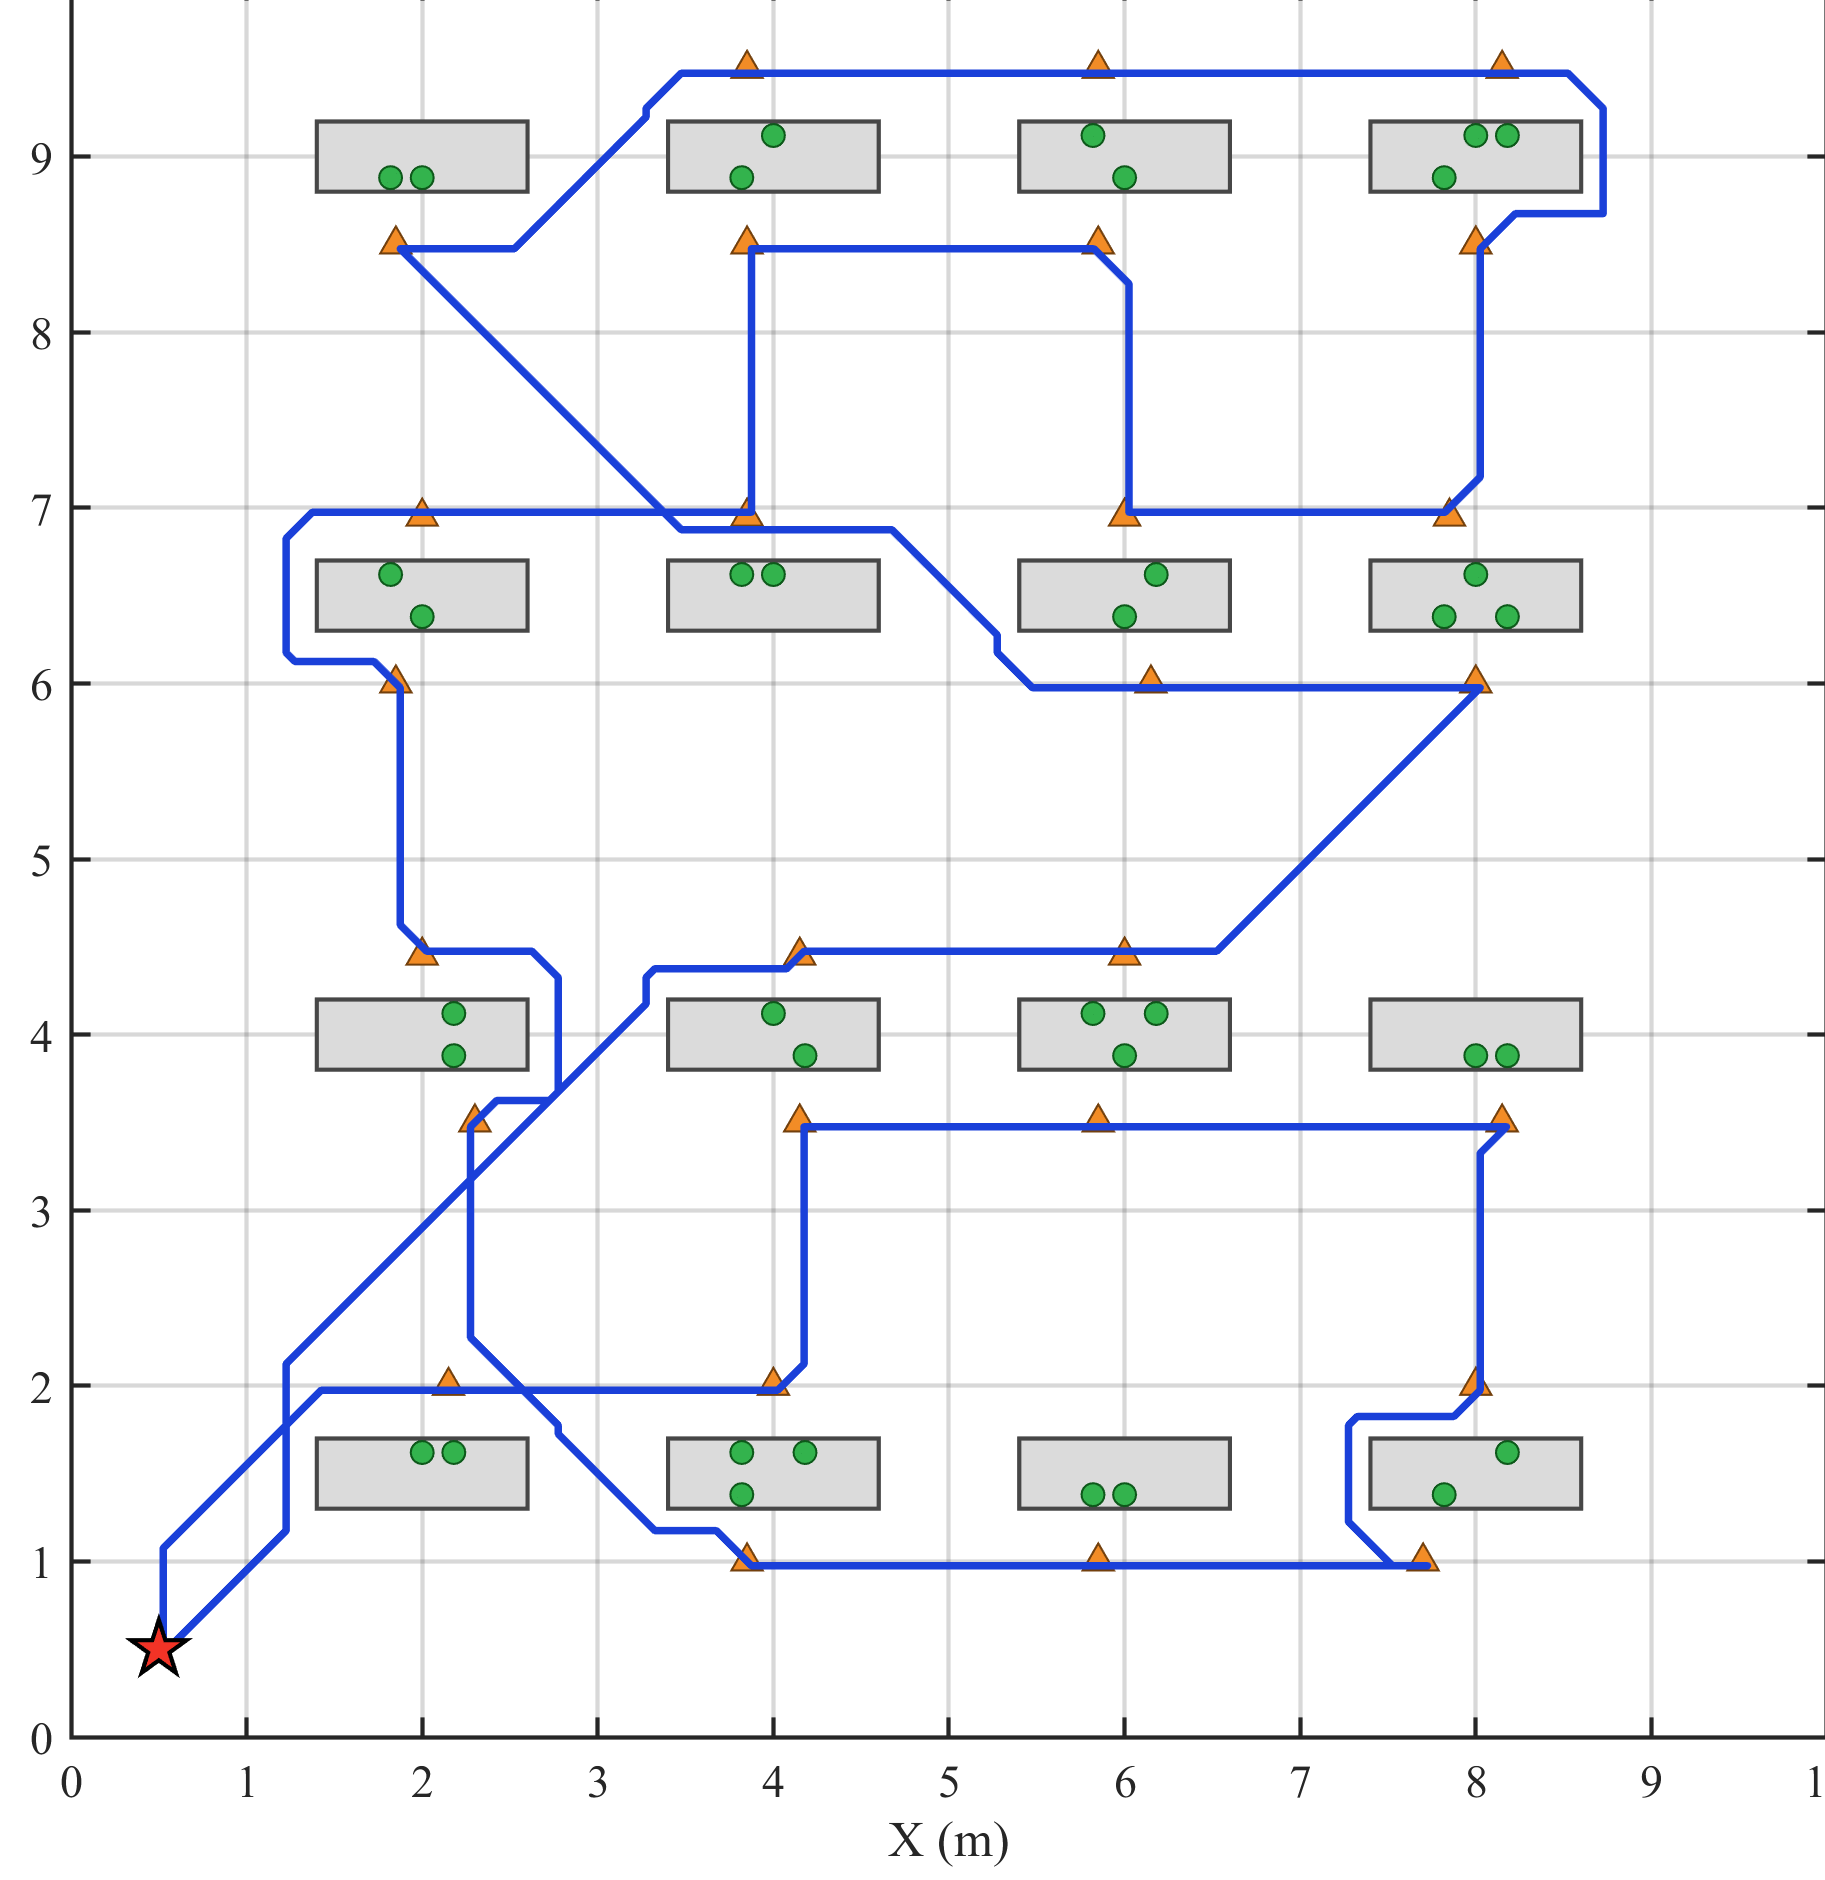
\includegraphics[width=0.88\columnwidth]{results/figures/tac_submission/png/fig_main_scenario_scene.png}
    \caption{Experimental configuration of the main tabletop-service scene. The \(10\,\mathrm{m}\times10\,\mathrm{m}\) 
    map contains 16 rectangular tables and 36 tabletop task points. Green circles mark tasks, 
    orange triangles mark selected collision-free docking poses, the red star marks the start state,
     and the blue polyline is the A*-planned route.}
    \label{fig:main_scenario_scene}
\end{figure}

\begin{figure*}[!t]
    \centering
    \begin{minipage}[t]{0.49\textwidth}
        \centering
        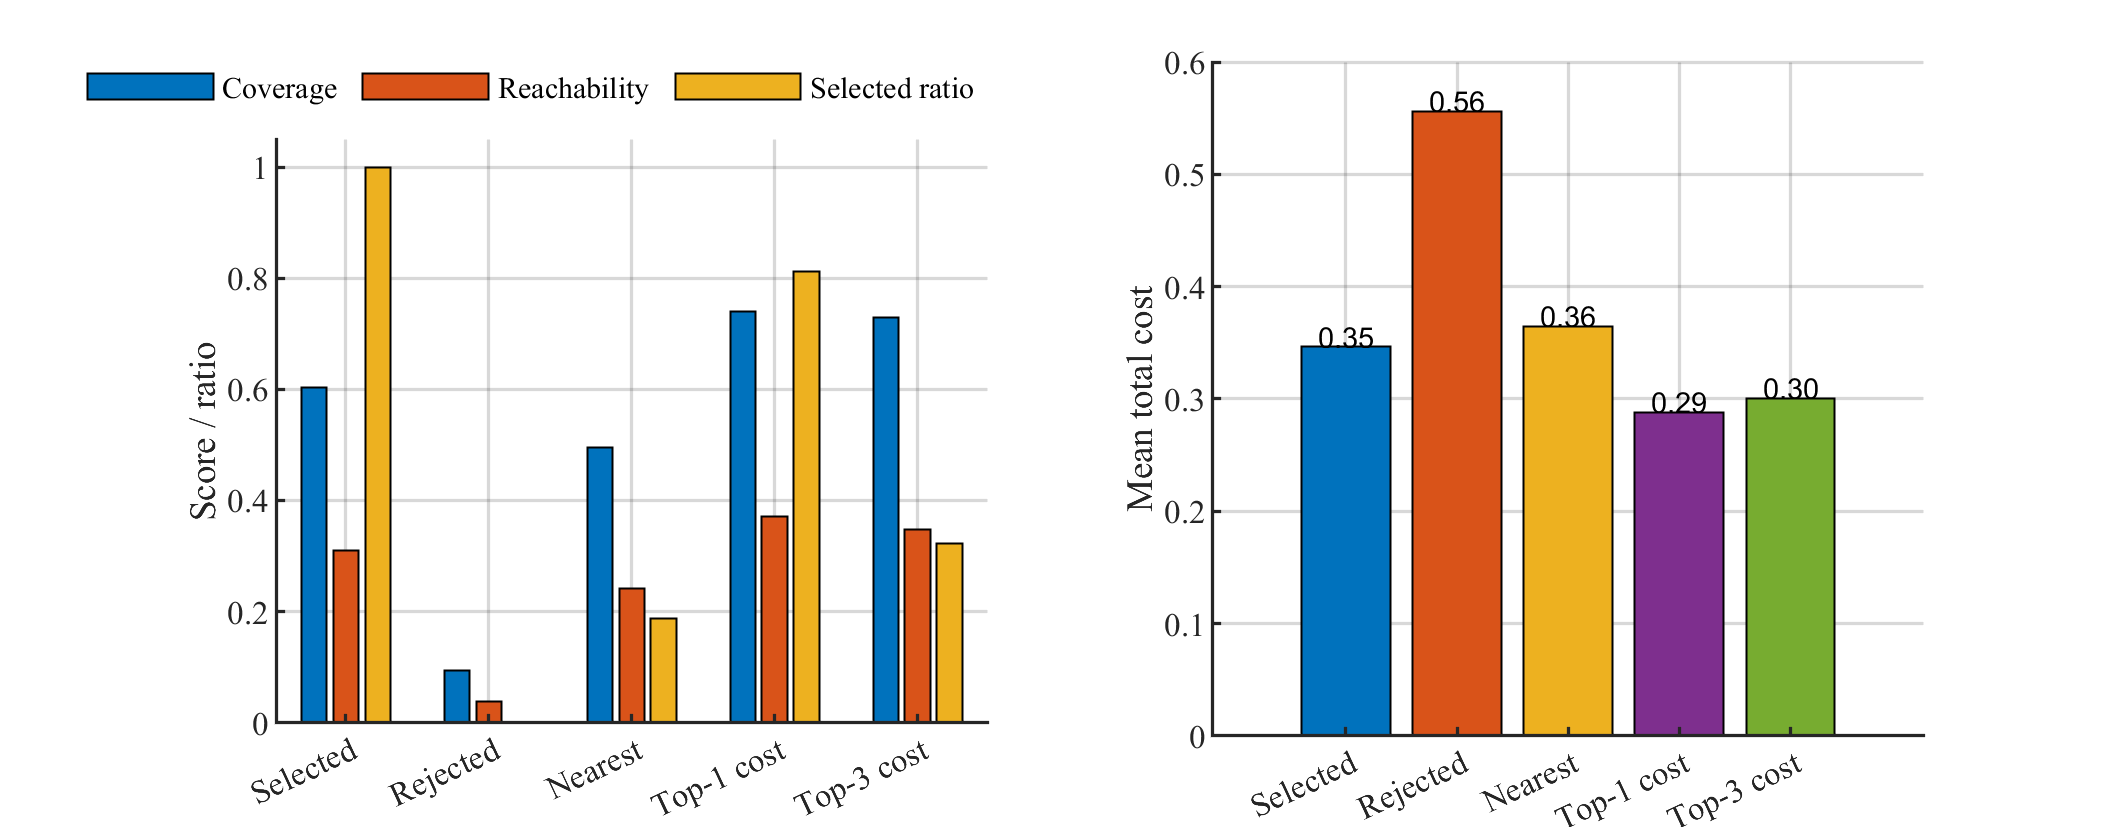
\includegraphics[width=\linewidth]{results/figures/tac_submission/png/fig_candidate_quality.png}
        \vspace{0.1em}
        \small (a) Candidate docking-pose quality.
    \end{minipage}\hfill
    \begin{minipage}[t]{0.49\textwidth}
        \centering
        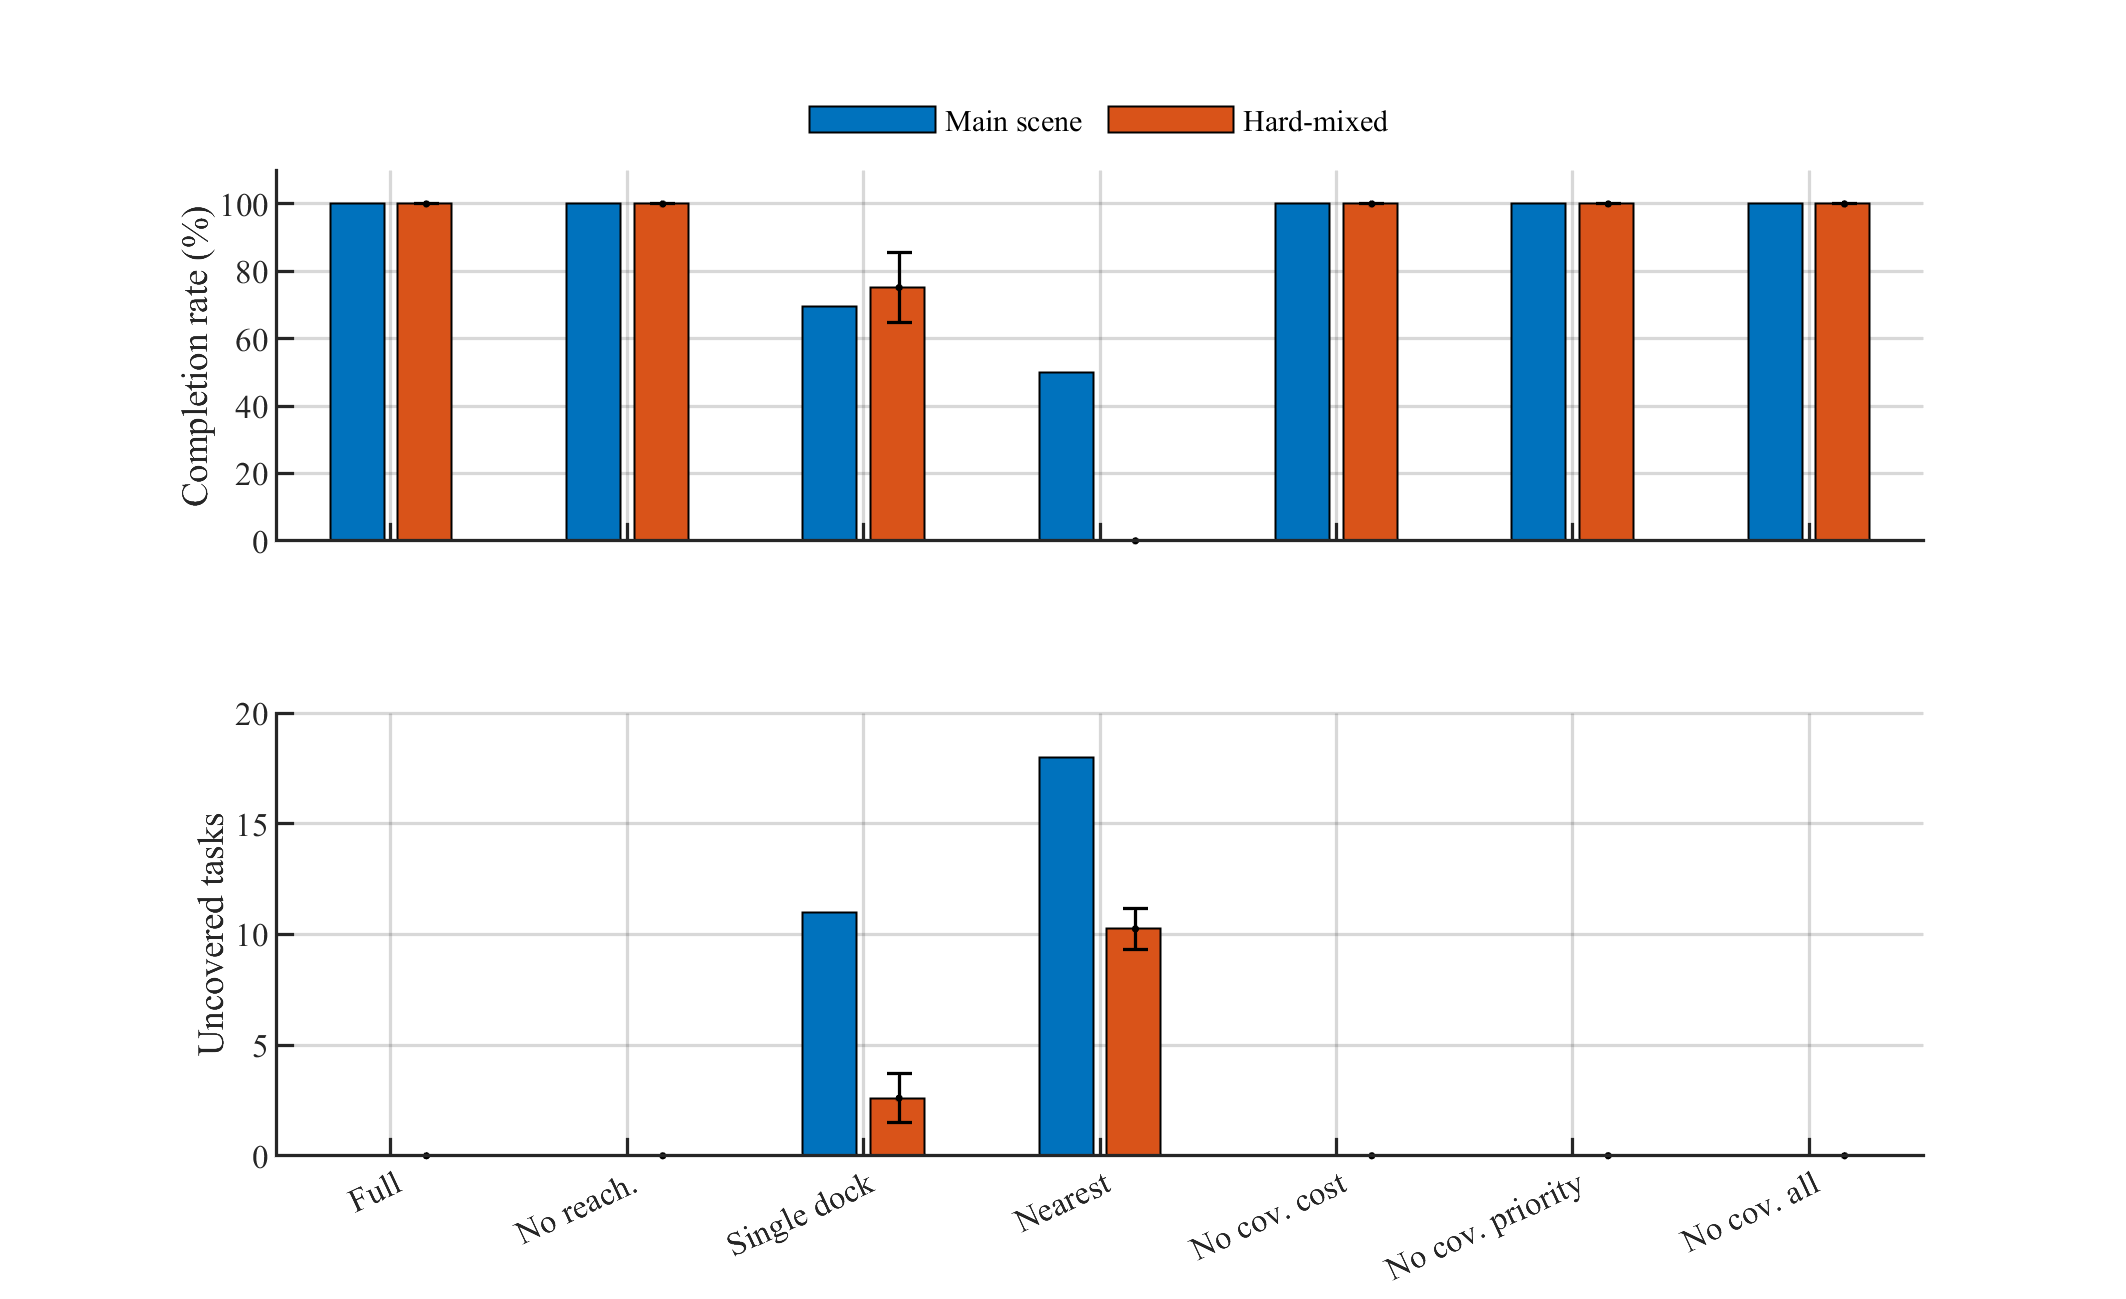
\includegraphics[width=\linewidth]{results/figures/tac_submission/png/fig_ablation_completion.png}
        \vspace{0.1em}
        \small (b) Main and hard-mixed ablations.
    \end{minipage}
    \caption{Candidate quality and ablation evidence. 
    (a) Selected poses provide stronger coverage and reachability than rejected candidates.
     (b) Single-docking and nearest-docking variants leave uncovered tasks 
     because they ignore either multi-side coverage or reachability-aware docking quality.}
    \label{fig:quality_ablation}
\end{figure*}

\begin{table}[!t]
\centering
\caption{Main scenario result.}
\label{tab:main}
\begin{tabular}{lr}
\toprule
Metric & Value \\
\midrule
Tasks & 36 \\
Completed tasks & 36 \\
Completion rate & 100.00\% \\
Selected docking poses & 27 \\
Task path length & 57.34 m \\
Return path length & 5.95 m \\
Total path length & 63.29 m \\
Planning time & 28.85 s \\
Estimated execution time & 789.79 s \\
\bottomrule
\end{tabular}
\end{table}

\subsection{Main Scenario and Candidate Quality}
    Table~\ref{tab:main} reports the numerical result for the scene in Figure~\ref{fig:main_scenario_scene}. 
    The full method completes all 36 tasks with 27 selected docking poses and a total route length of 63.29 m. 
    This result supports the central claim that tabletop service requirements can first be converted into 
    reachability-aware docking decisions and then connected by a replaceable global path planner. 
    The relatively large number of selected poses is not a failure of path shortening; it reflects 
    the manipulation constraint that some tables require service from multiple sides to cover all task points.

    Figure~\ref{fig:quality_ablation}(a) compares selected and rejected candidate docking poses. 
    Selected candidates have mean coverage ratio 0.604 and mean reachability score 0.310,
    while rejected candidates have mean coverage ratio 0.094 and mean reachability score 0.038. 
    This gap indicates that the scoring function selects poses that are meaningfully better for 
    manipulation coverage rather than merely close in navigation space.

\subsection{Ablation Studies}
Figure~\ref{fig:quality_ablation}(b) and Table~\ref{tab:baseline_submission} evaluate the necessity of reachability-aware multi-docking. 
In the main scenario, the full method reaches 100.00\% completion, while single docking per table reaches 69.44\% and nearest docking reaches 50.00\%. 
In the submission-level baseline comparison over 1120 records, the full method keeps 100.00\% mean completion, single docking reaches 73.73\%, 
and nearest docking reaches 25.59\%. 
These failures show that shorter or simpler docking choices are not sufficient when task coverage is constrained by dual-arm reachability.

\begin{table}[!t]
\centering
\caption{Submission-level baseline comparison.}
\label{tab:baseline_submission}
\footnotesize
\setlength{\tabcolsep}{3.2pt}
\begin{tabular}{@{}lrrrrr@{}}
\toprule
Method & Trials & Completion & Uncovered & Docks & Time \\
 & & (\%) & & & (s) \\
\midrule
Full & 140 & 100.00 & 0.00 & 10.99 & 12.28 \\
Single dock & 140 & 73.73 & 4.49 & 6.43 & 11.10 \\
Nearest & 120 & 25.59 & 10.99 & 6.83 & 11.17 \\
Set-cover greedy & 140 & 100.00 & 0.00 & 11.11 & 10.62 \\
Random feasible & 140 & 100.00 & 0.00 & 15.02 & 13.05 \\
\bottomrule
\end{tabular}
\end{table}

\subsection{Hard Scenarios and Stress Boundaries}
 The hard-scenario suite includes normal, hard-corner, hard-two-side, hard-reach-boundary, 
 and hard-mixed task distributions. The full method maintains complete coverage in all five distributions in the generated summary data. 
 Figure~\ref{fig:hard_stress}(a) shows that nearest and single-docking baselines degrade sharply under hard distributions, 
 which supports the need for multi-docking coverage.
 Figure~\ref{fig:hard_stress}(b) reports sensitivity to table spacing, reachability threshold, task density, and candidate density. 
 The lowest mean completion in the stress summary is 96.92\% at reachability threshold 0.5,
  while most settings remain at full completion.

\begin{figure*}[!t]
    \centering
    \begin{minipage}[t]{0.49\textwidth}
        \centering
        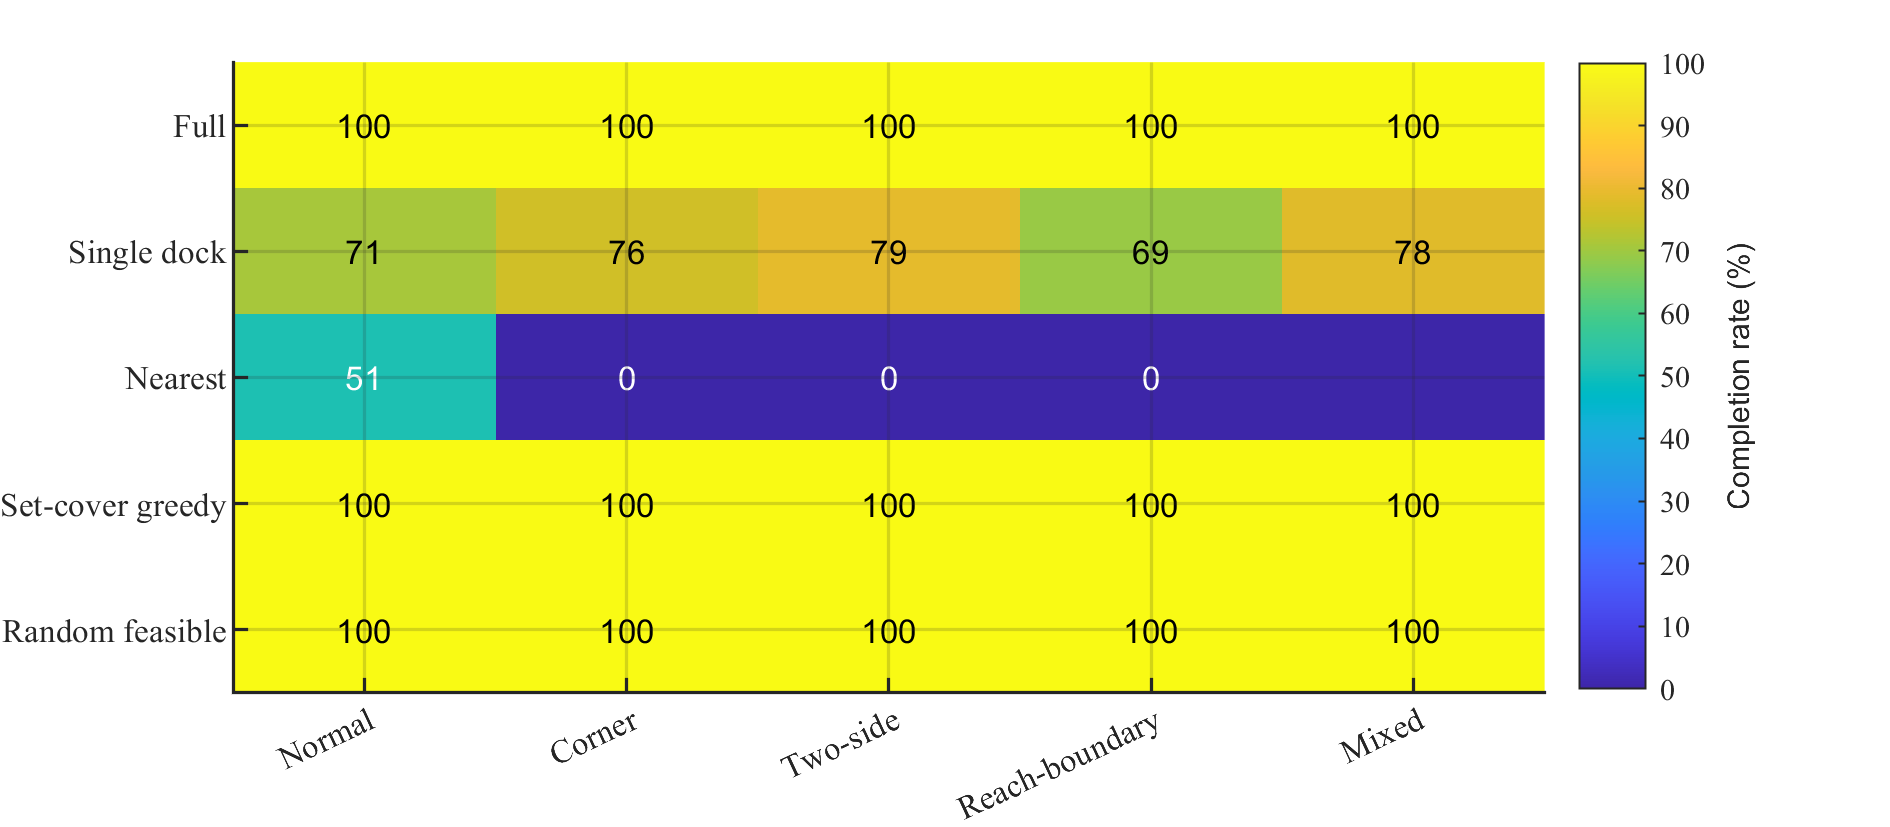
\includegraphics[width=\linewidth]{results/figures/tac_submission/png/fig_hard_scenario_heatmap.png}
        \vspace{0.2em}
        \small (a) Completion across hard distributions.
    \end{minipage}\hfill
    \begin{minipage}[t]{0.49\textwidth}
        \centering
        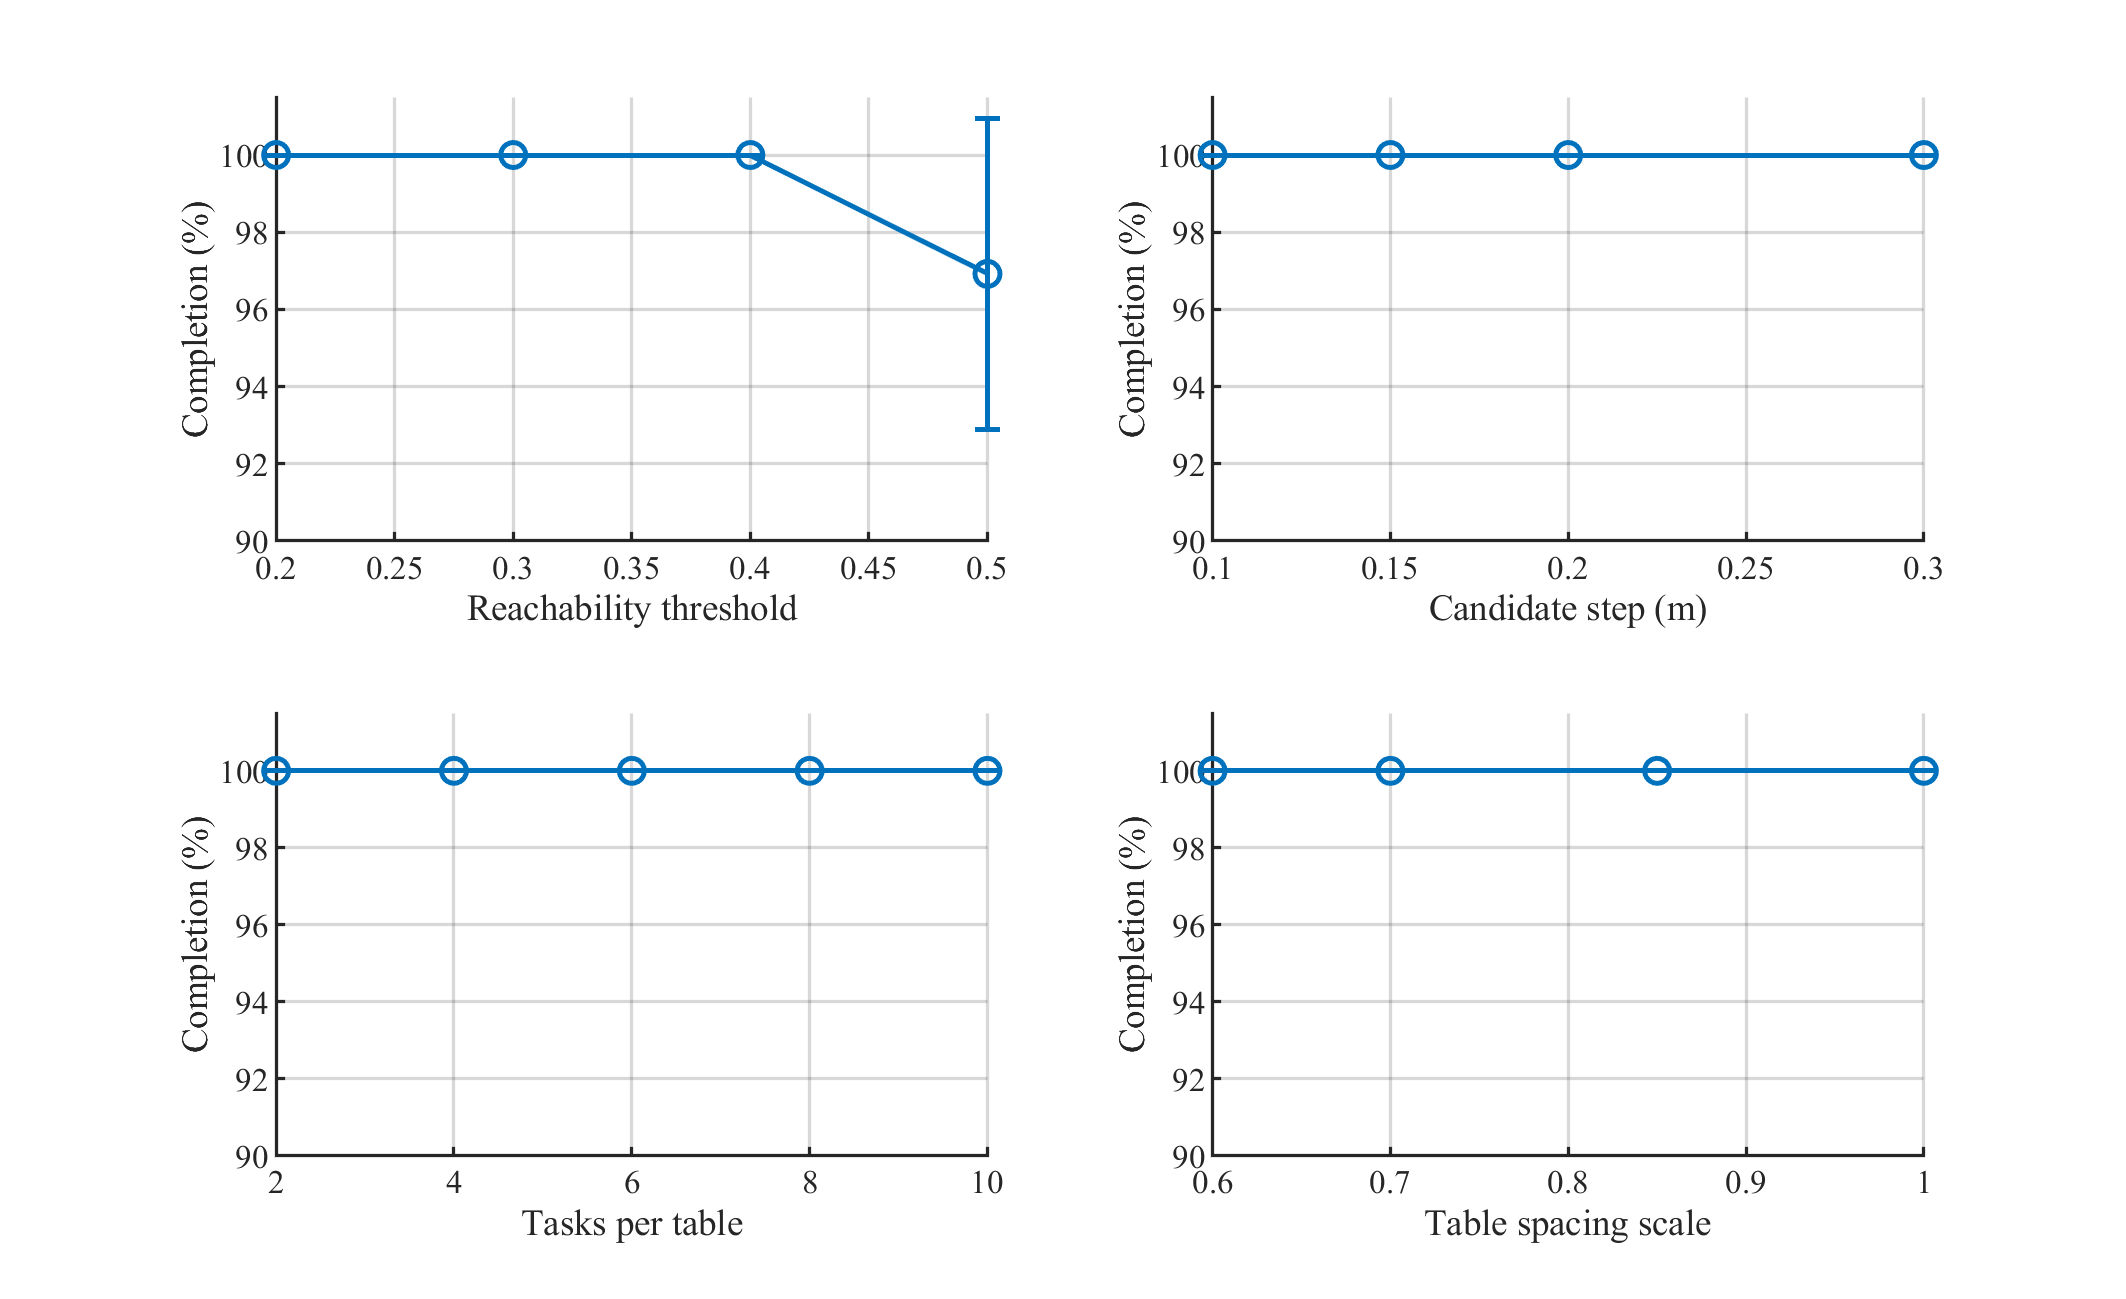
\includegraphics[width=\linewidth]{results/figures/tac_submission/png/fig_stress_boundary.png}
        \vspace{0.2em}
        \small (b) Boundary and sensitivity scans.
    \end{minipage}
    \caption{Robustness under difficult task distributions and parameter stress. 
    The full method remains stable across hard scenarios, while tighter reachability 
    constraints are the main source of completion degradation in the stress scan.}
    \label{fig:hard_stress}
\end{figure*}

\subsection{Runtime Scaling and Noise Robustness}
Figure~\ref{fig:runtime_routing1}(a) shows planning-time trends across scale and candidate-density settings.
 Planning time ranges from 1.92 s to 60.02 s in the submission summary, 
 consistent with the \(O(KN)\) candidate-evaluation term and the \(O(Q^2 C_{\Pi})\) pairwise path-cost term in Proposition~\ref{prop:complexity}.
  Figure~\ref{fig:runtime_routing1}(b) reports perturbation tests. 
  The full method's final completion ranges from 69.03\% to 100.00\% across noise settings,
   while the nearest-docking baseline remains at 0.00\% in the same summary.


\subsection{Global Planner Benchmark and Oracle Reference}
 Figure~\ref{fig:runtime_routing1}(c) compares global planners under the same selected docking sequence. 
 All seven planners succeed, with path-length and turn-count differences reflecting 
 the routing module rather than the docking selection module.
 A* gives 63.29 m, JPS gives 63.24 m, GBFS gives 66.47 m, Theta* gives 62.46 m, Lazy Theta* gives 62.87 m, 
 and Convex A* gives 63.29 m in the fixed-order benchmark. 
 Figure~\ref{fig:runtime_routing1}(d) compares the heuristic with a small-scale bounded candidate-set oracle. 
 The relative gap ranges from -4.56\% to 0.63\%; 
 negative gaps arise from the restricted comparison objective and 
 should be interpreted as a consistency check rather than a proof of global optimality. 

% \twocolumn[{
%     \begin{center}
%     \begin{minipage}[t]{0.49\textwidth}
%         \centering
%         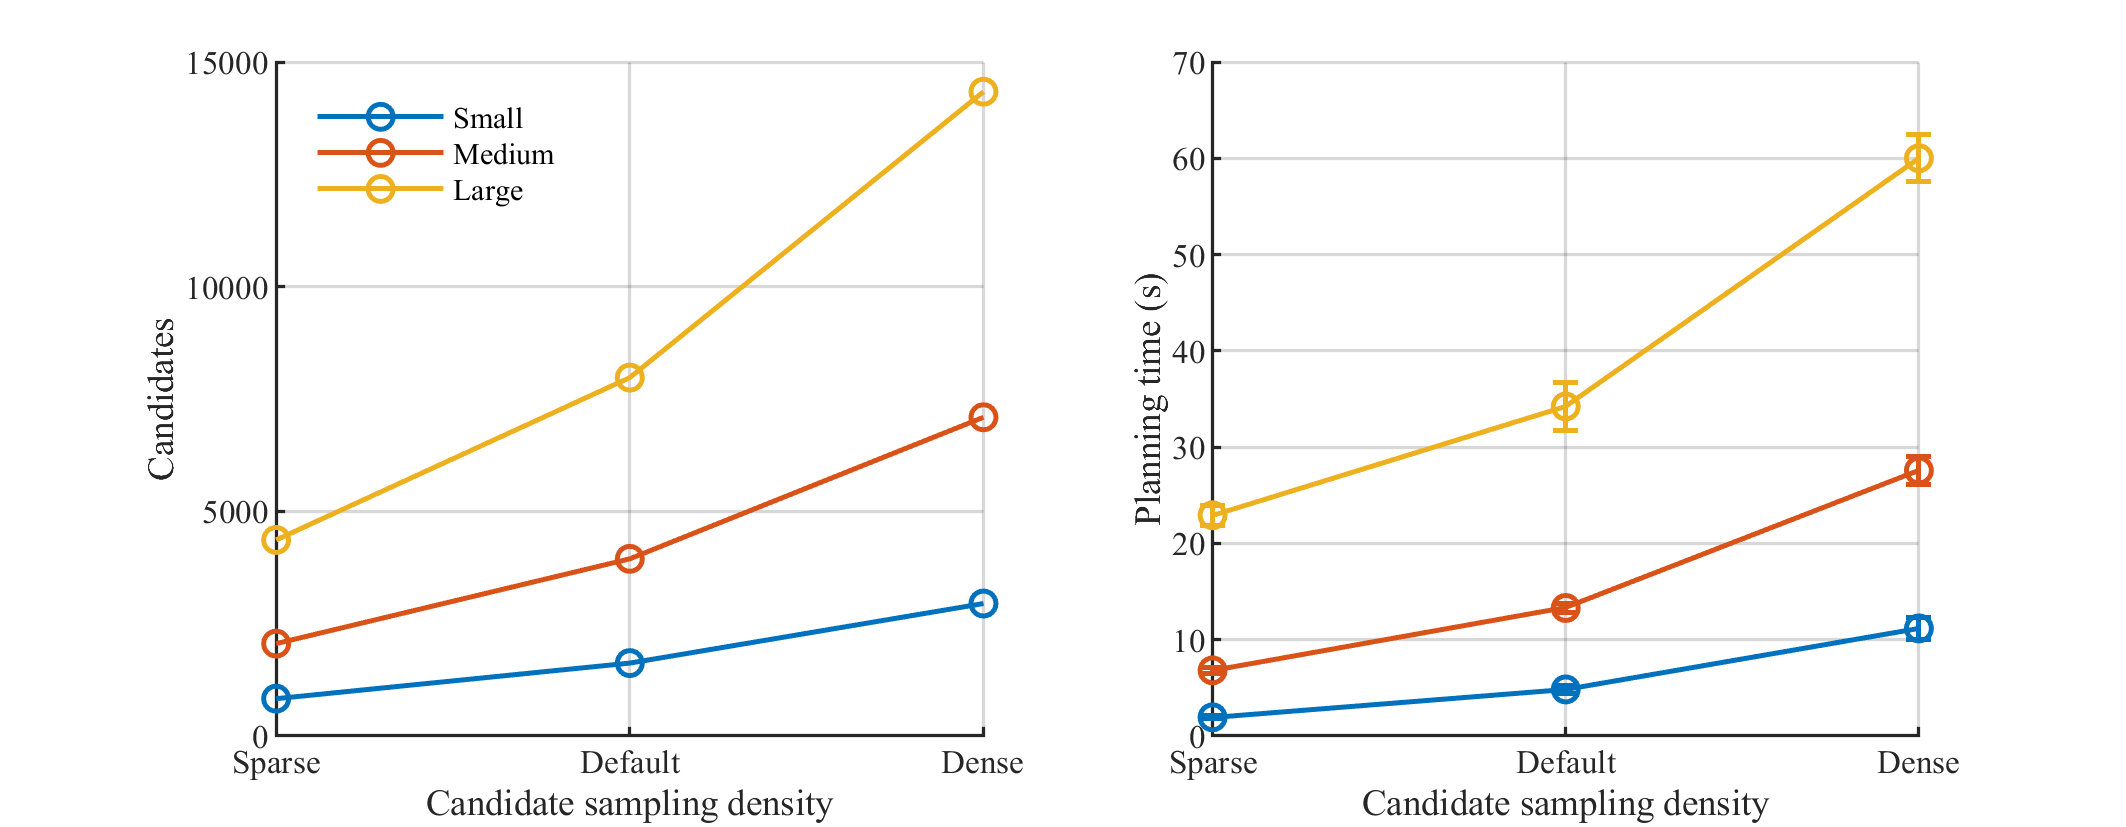
\includegraphics[width=\linewidth]{results/figures/tac_submission/png/fig_runtime_scaling.png}
%         \vspace{0.2em}
%         \small (a) Runtime scaling.
%     \end{minipage}\hfill
%     \begin{minipage}[t]{0.49\textwidth}
%         \centering
%         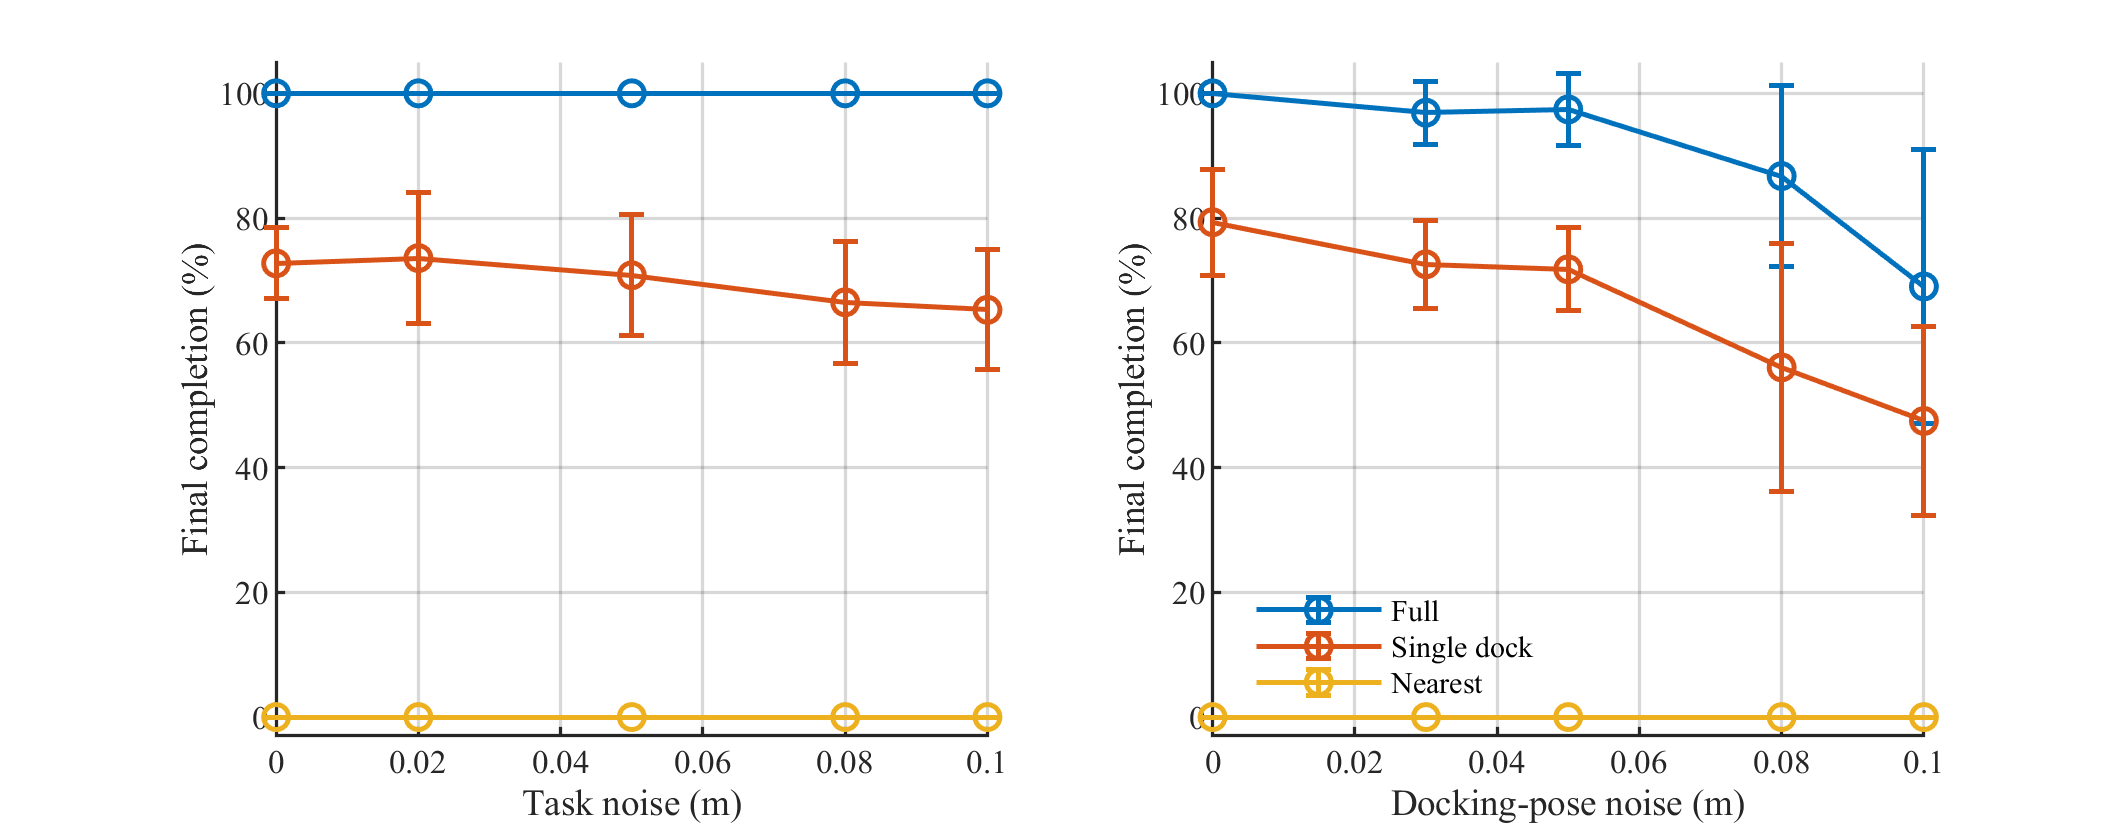
\includegraphics[width=\linewidth]{results/figures/tac_submission/png/fig_noise_robustness.png}
%         \vspace{0.2em}
%         \small (b) Noise robustness.
%     \end{minipage}
%     \vspace{0.5em}

%     \begin{minipage}[t]{0.49\textwidth}
%         \centering
%         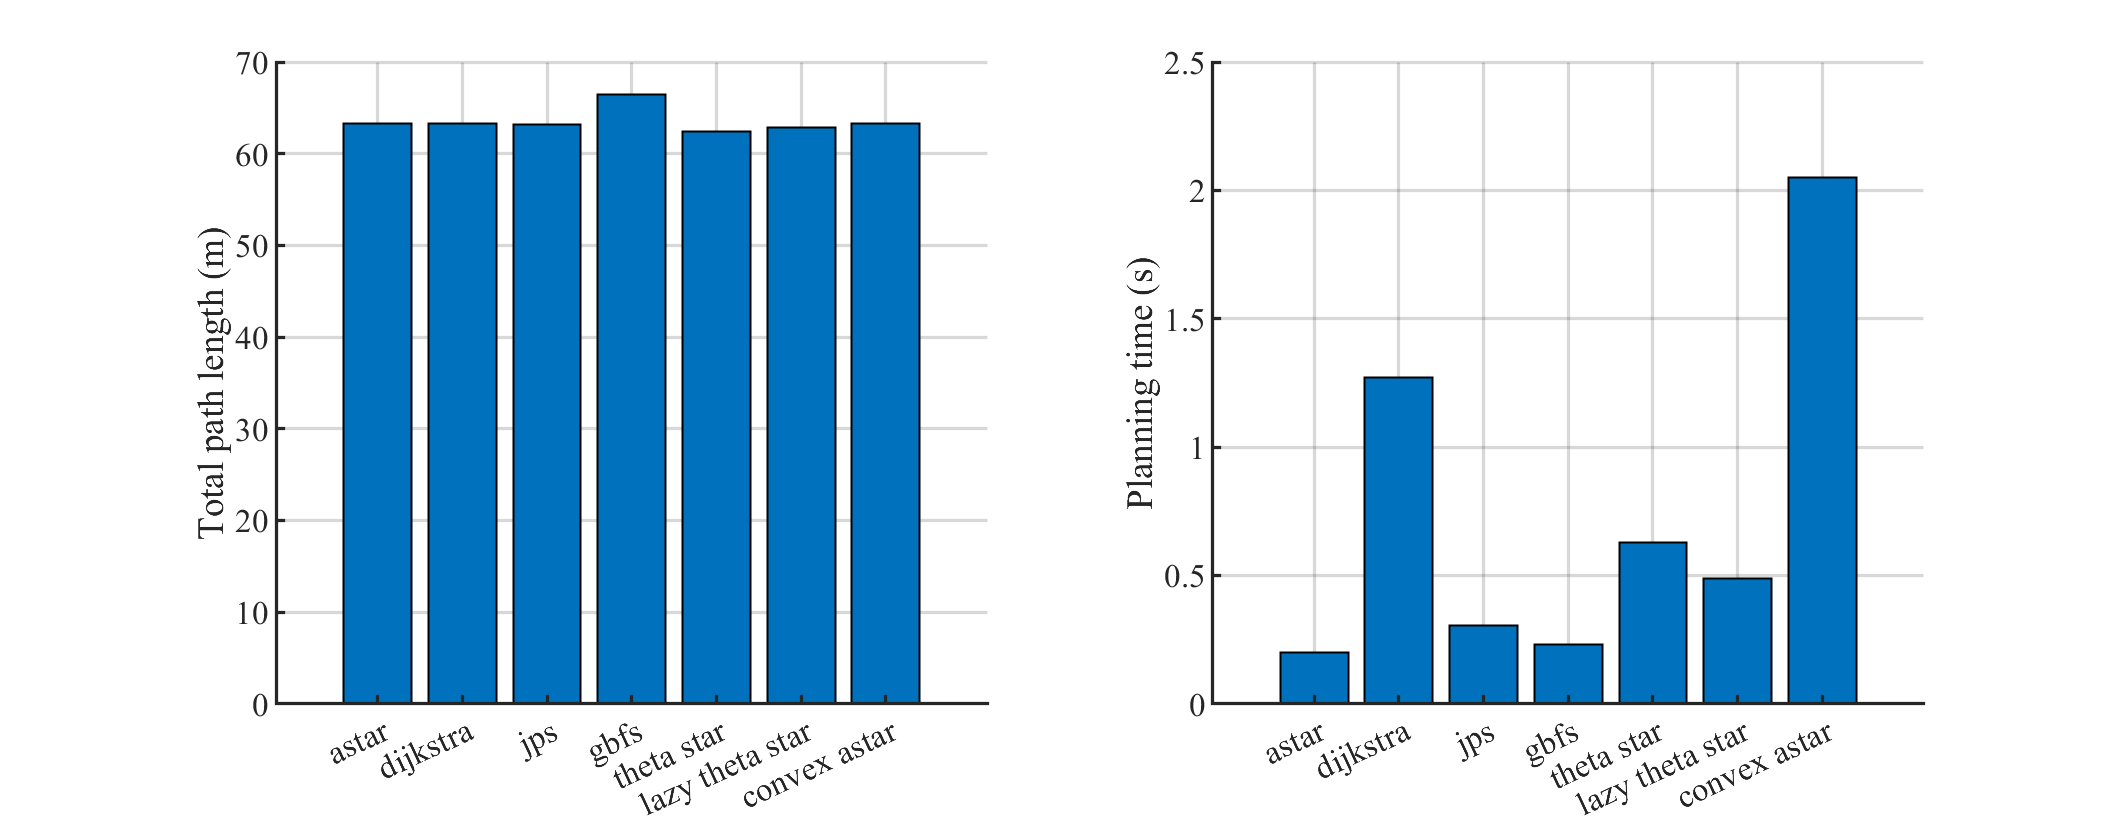
\includegraphics[width=\linewidth]{results/figures/tac_submission/png/fig_global_planner_benchmark.png}
%         \vspace{0.2em}
%         \small (c) Global planner benchmark.
%     \end{minipage}\hfill
%     \begin{minipage}[t]{0.49\textwidth}
%         \centering
%         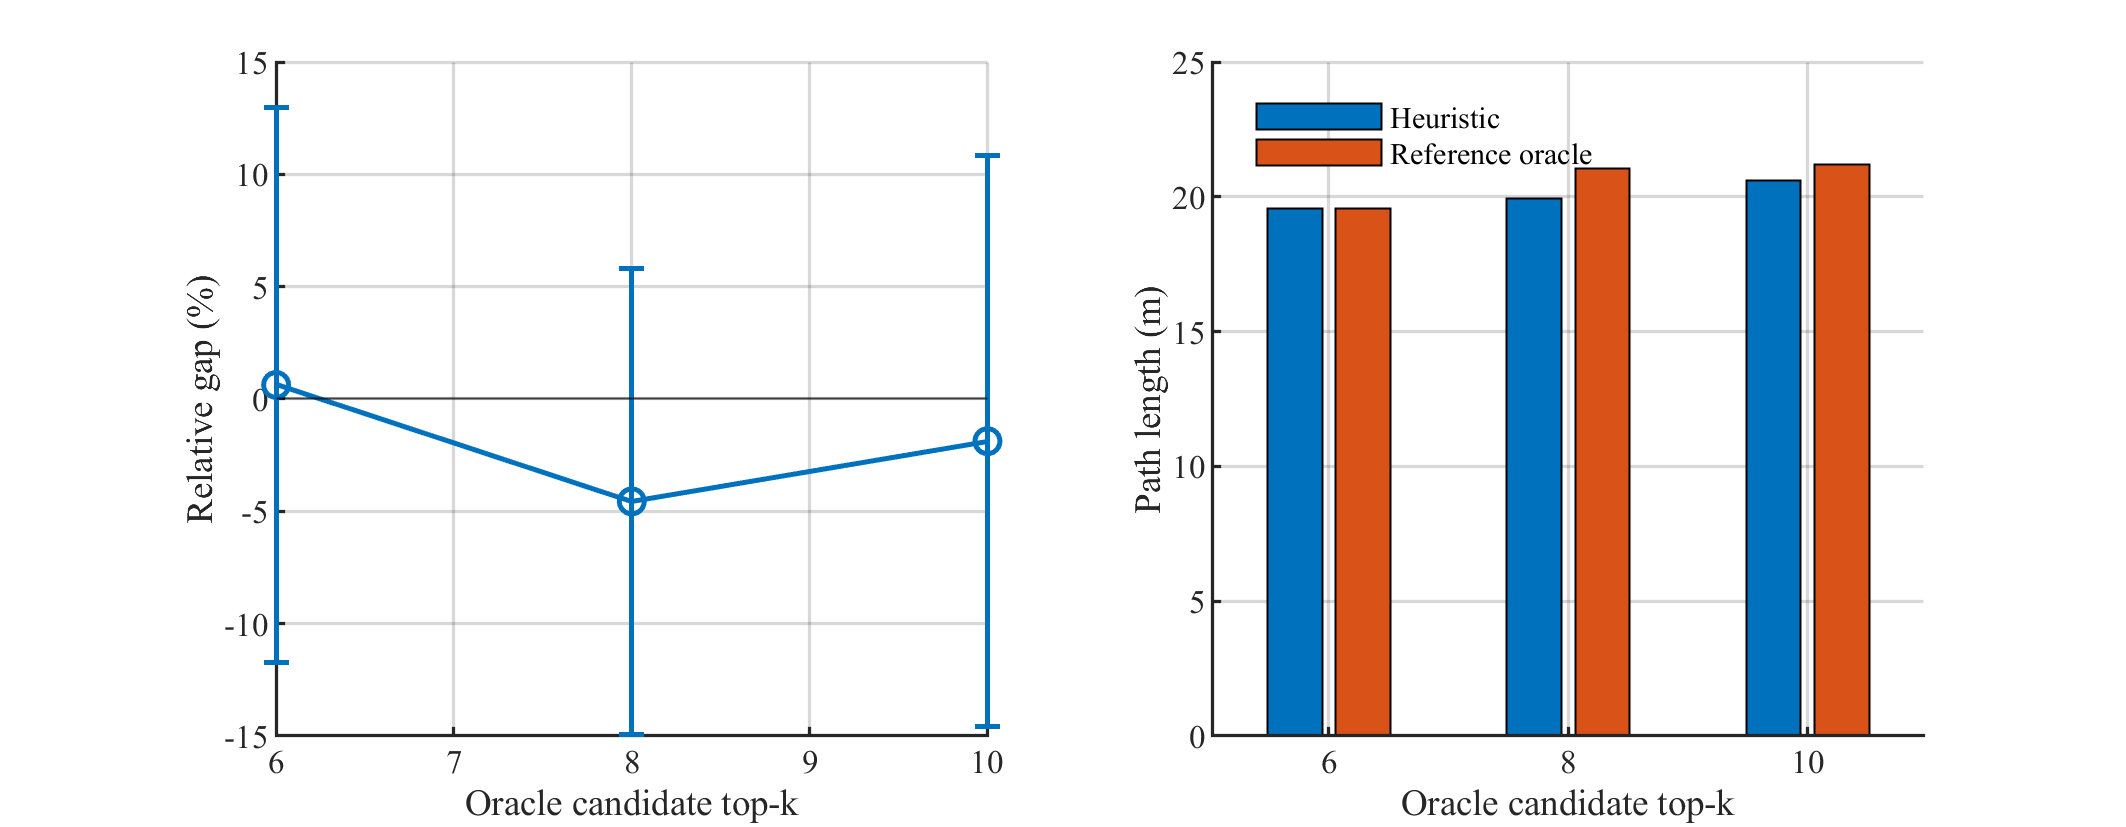
\includegraphics[width=\linewidth]{results/figures/tac_submission/png/fig_oracle_gap.png}
%         \vspace{0.2em}
%         \small (d) Small-scale oracle reference.
%     \end{minipage}
%     \refstepcounter{figure}\label{fig:runtime_routing}
%     \vspace{0.3em}

%     \parbox{0.96\textwidth}{\footnotesize \textbf{Fig.~\thefigure.} 
%      Runtime, perturbation, routing, 
%      and oracle-reference results. Runtime increases with scene scale and candidate density; 
%      reachability-aware coverage improves robustness under perturbations; 
%      changing the global planner affects route properties without changing docking selection;
%      and the heuristic remains close to the bounded candidate-set oracle on reduced instances.}
%     \end{center}
%     \vspace{0.6em}
% }]

\begin{figure*}[!t]
    \centering
    \begin{minipage}[t]{0.49\textwidth}
        \centering
        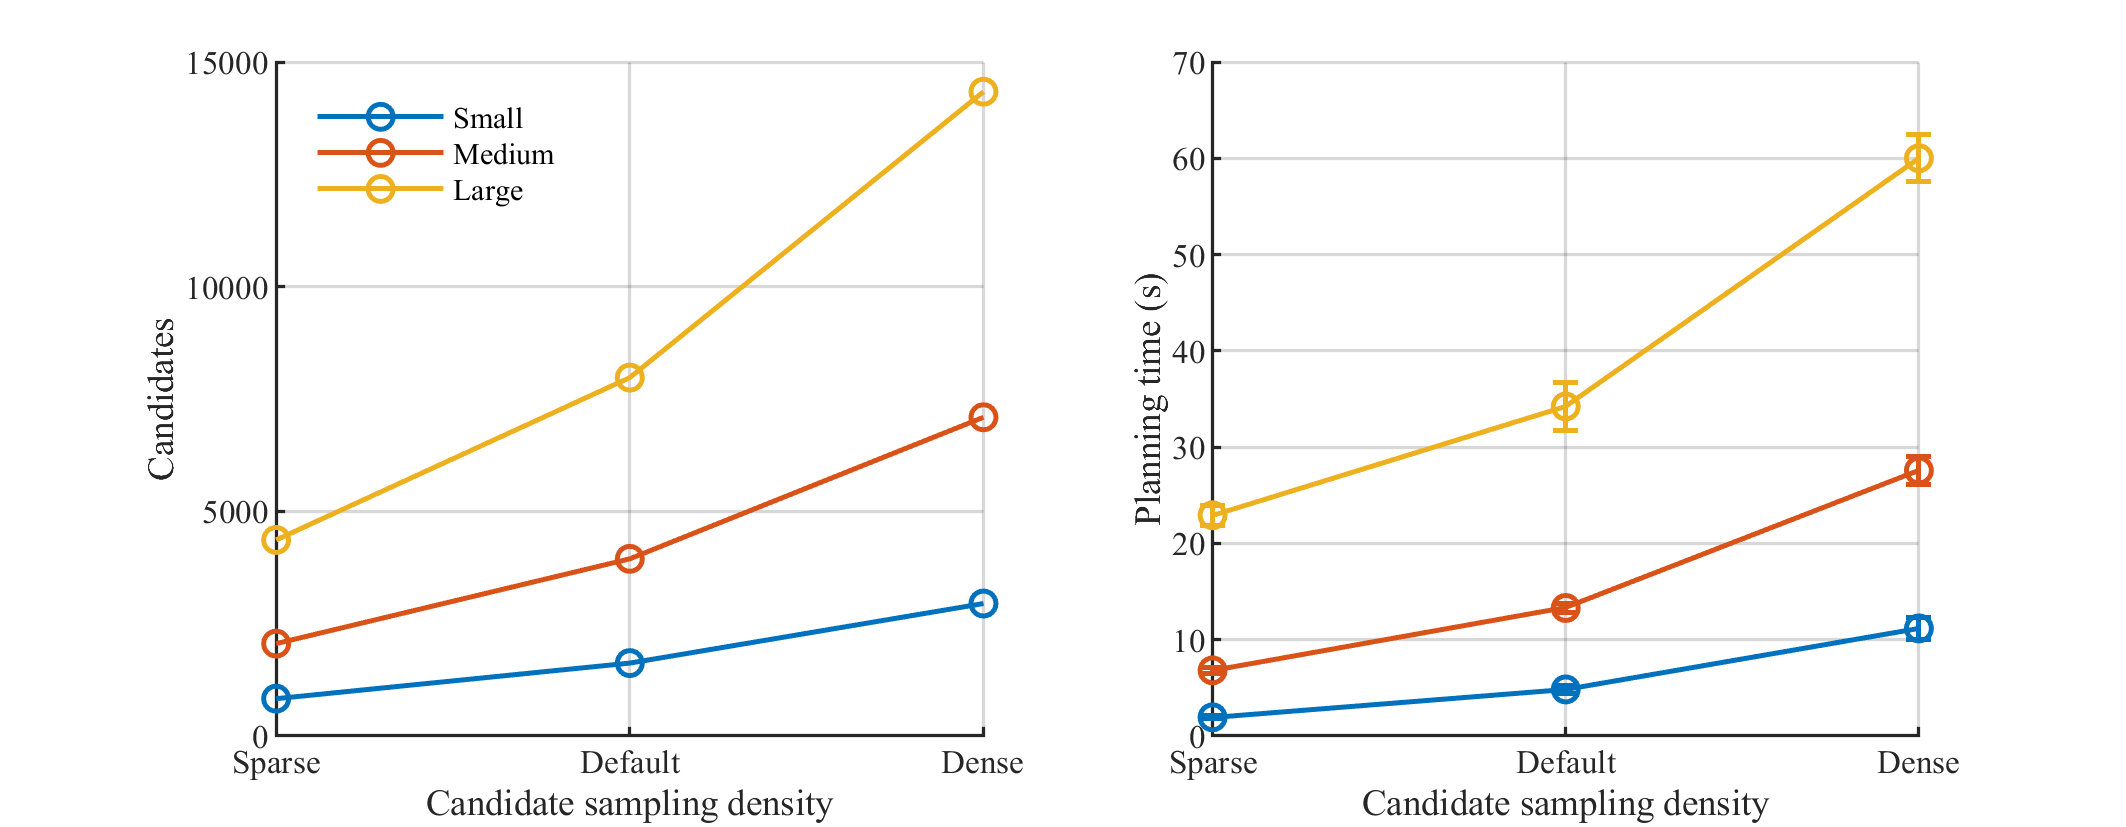
\includegraphics[width=\linewidth]{results/figures/tac_submission/png/fig_runtime_scaling.png}
        \vspace{0.2em}
        \small (a) Global planner benchmark.
    \end{minipage}\hfill
    \begin{minipage}[t]{0.49\textwidth}
        \centering
        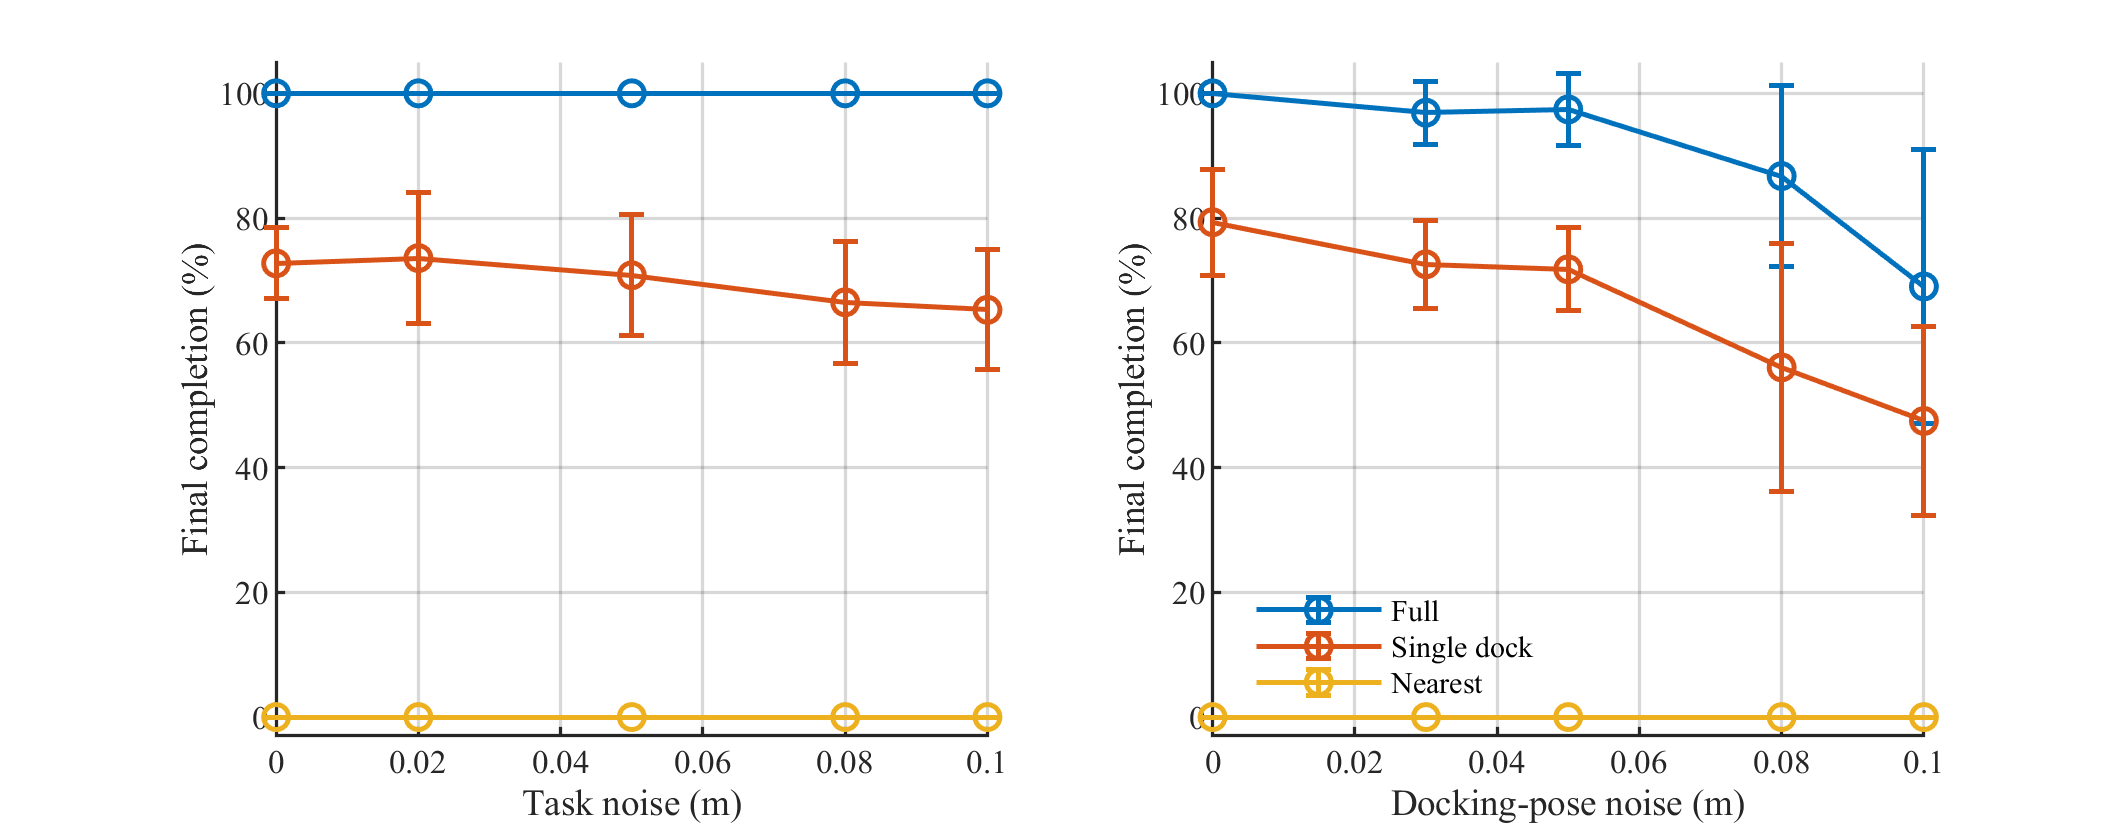
\includegraphics[width=\linewidth]{results/figures/tac_submission/png/fig_noise_robustness.png}
        \vspace{0.2em}
        \small (b) Small-scale oracle reference.
    \end{minipage}
    \caption{Robustness under difficult task distributions and parameter stress. 
    The full method remains stable across hard scenarios, while tighter reachability 
    constraints are the main source of completion degradation in the stress scan.}
    \label{fig:runtime_routing1}
\end{figure*}

\begin{figure*}[!t]
    \centering
    \begin{minipage}[t]{0.49\textwidth}
        \centering
        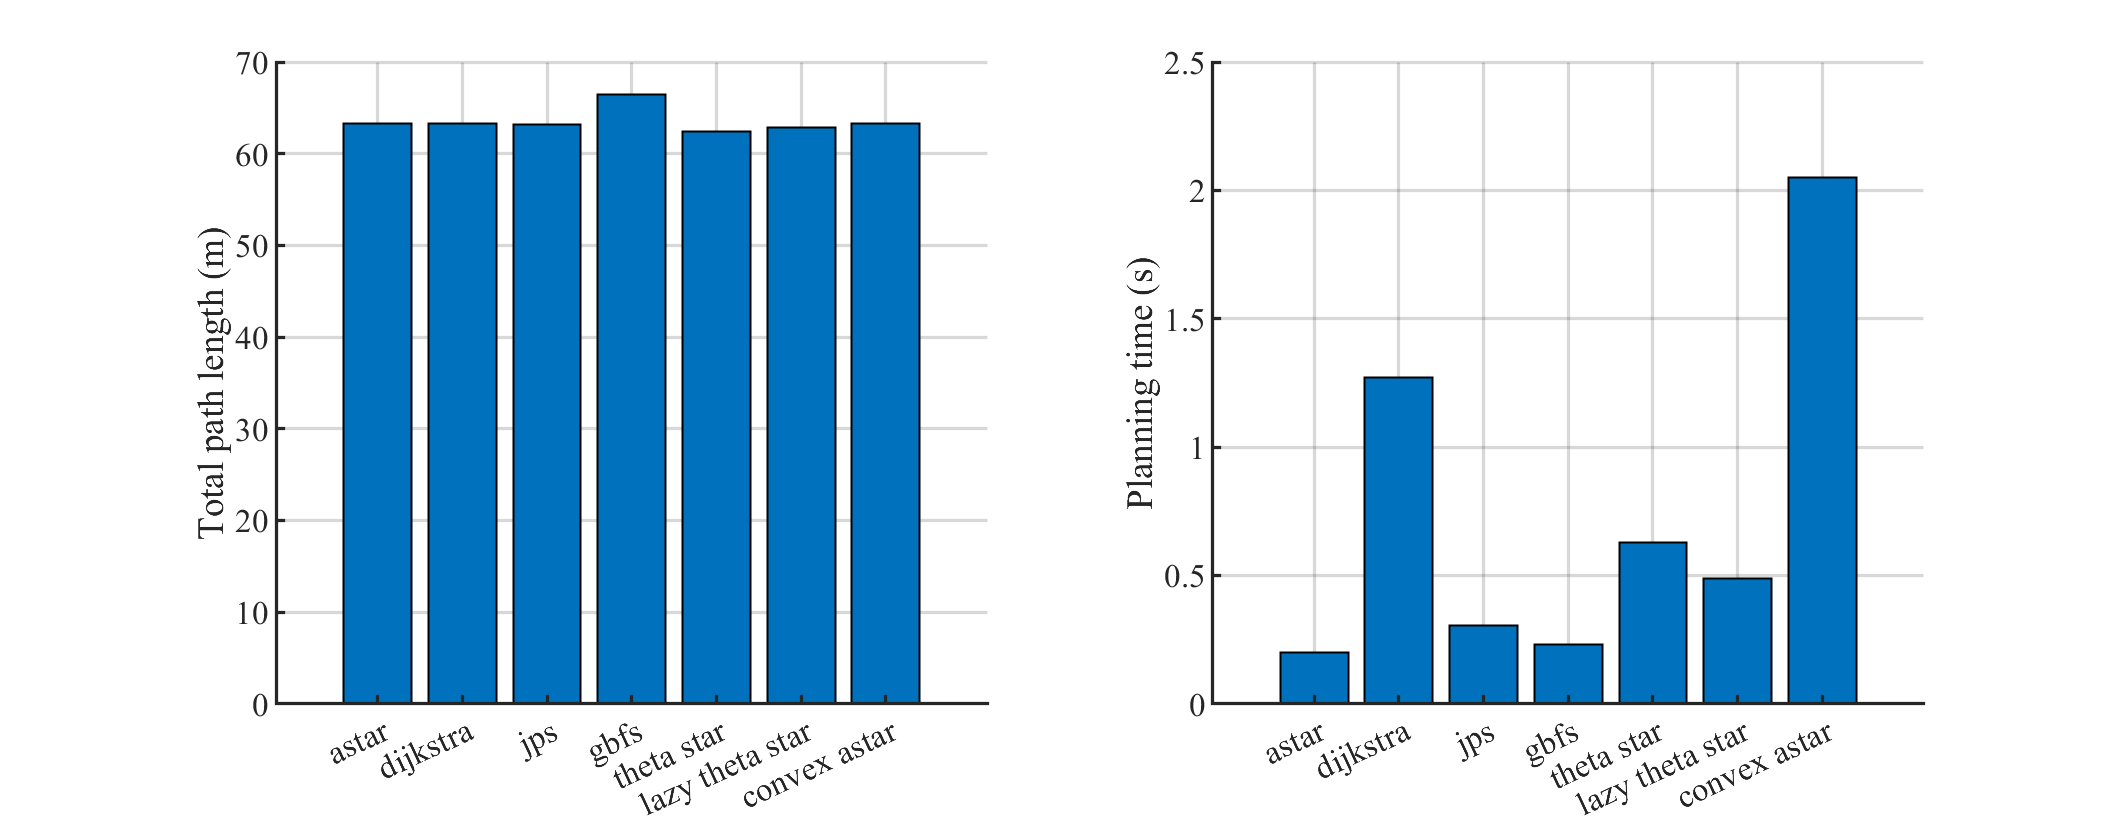
\includegraphics[width=\linewidth]{results/figures/tac_submission/png/fig_global_planner_benchmark.png}
        \vspace{0.2em}
        \small (a) Global planner benchmark.
    \end{minipage}\hfill
    \begin{minipage}[t]{0.49\textwidth}
        \centering
        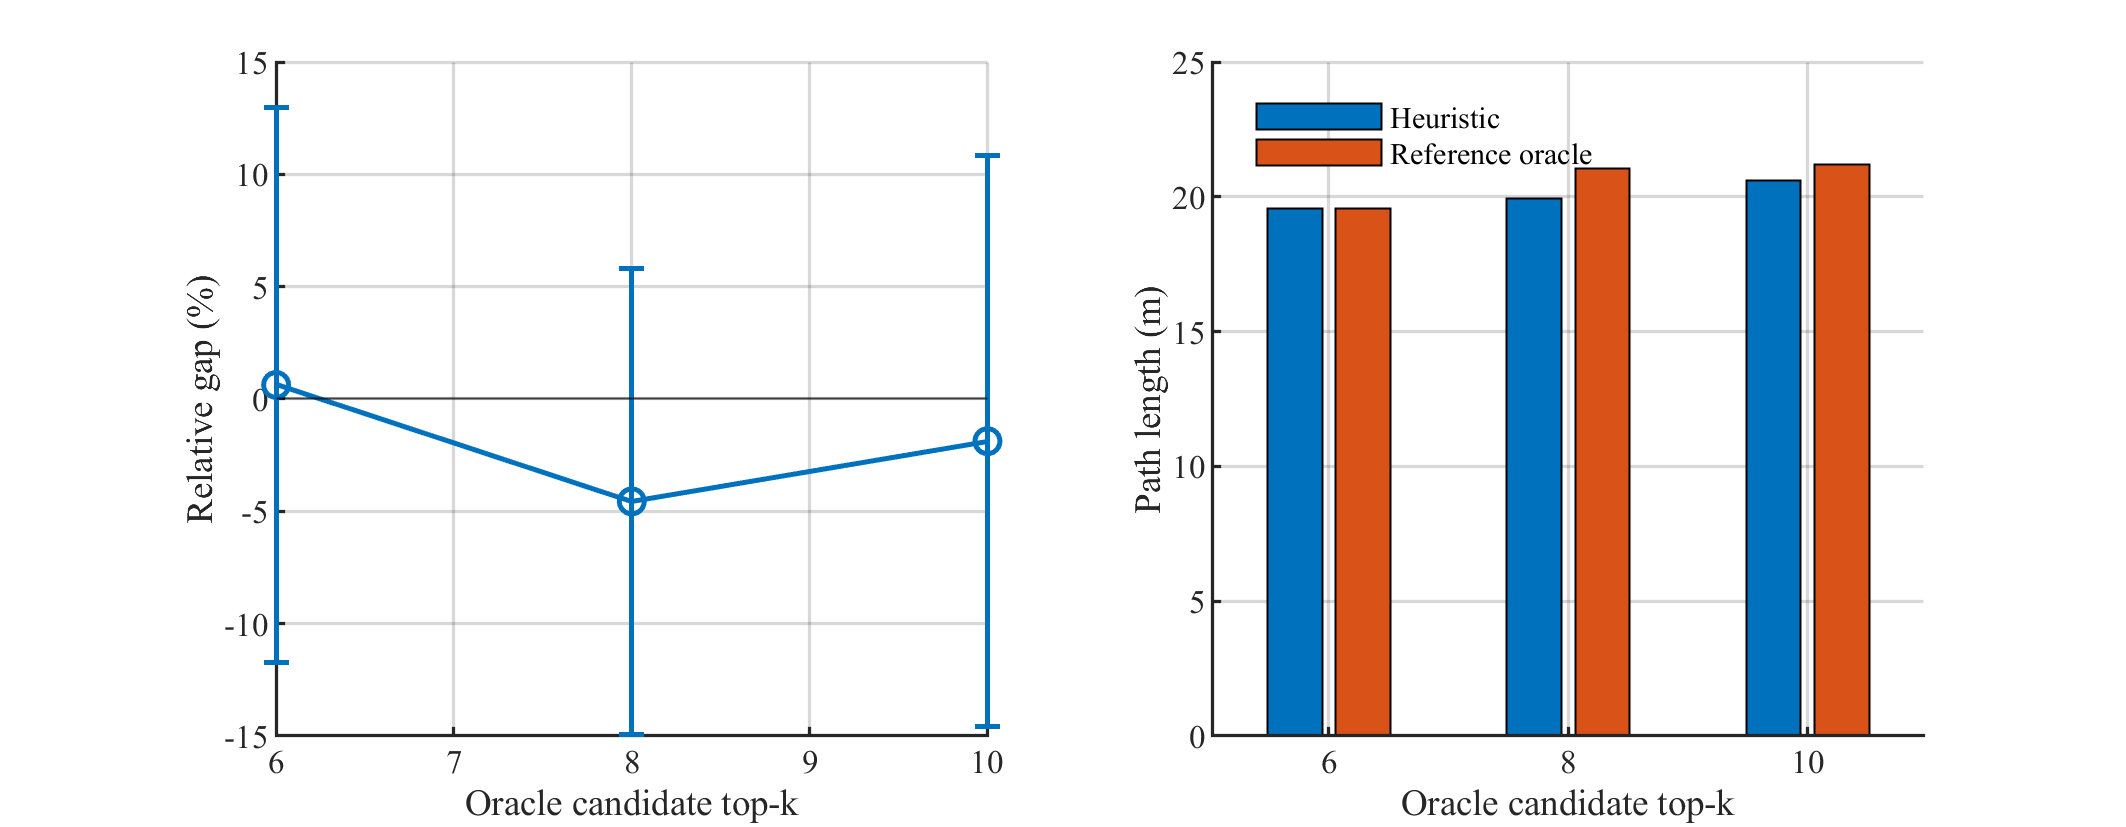
\includegraphics[width=\linewidth]{results/figures/tac_submission/png/fig_oracle_gap.png}
        \vspace{0.2em}
        \small (b) Small-scale oracle reference.
    \end{minipage}
    \caption{Robustness under difficult task distributions and parameter stress. 
    The full method remains stable across hard scenarios, while tighter reachability 
    constraints are the main source of completion degradation in the stress scan.}
    \label{fig:runtime_routing2}
\end{figure*}




\section{Conclusion}
\label{sec:conclusion}

This paper presented RCH-MT-MMP, a constrained hierarchical planning framework for reachability-aware multi-task mobile manipulation. The method treats tabletop task points as manipulation targets that must first be mapped to reachable docking-pose coverage sets. A coverage-aware multi-docking strategy then jointly covers complex table tasks, and a replaceable global planner connects the selected poses. The feasibility and complexity analysis clarifies when full coverage is guaranteed and where computation is spent. Experiments show that the full method maintains complete task coverage in the main and hard scenarios, while nearest and single-docking baselines fail under reachability-constrained task distributions.

The present results are based on known 2-D maps, simplified reachability scoring, and offline planning. Future work should integrate full manipulator dynamics, online perception, replanning under moving obstacles, and real-robot validation to connect the decision layer with closed-loop mobile-manipulation execution.


% \appendices
% \section{Additional Experimental Details}
\label{app:details}

The submission data used in this draft are indexed by the evidence report in \path{results/tables/tac_submission/tac_evidence_index_submission.csv}. The table groups include experiment parameters, main scenario summaries, candidate-quality summaries, hard-scenario summaries, main and hard ablations, random-scale studies, global-planner benchmarks, extended baselines, stress-boundary scans, runtime-scaling studies, noise-robustness tests, and small-scale oracle references.

\section{Reproducibility Notes}
\label{app:reproducibility}

The MATLAB entry point for regenerating the submission-level data is
\begin{verbatim}
run_tac_data_support('submission')
\end{verbatim}
The paper figures are generated under
\begin{verbatim}
results/figures/tac_submission/
\end{verbatim}
and the summary tables are generated under
\begin{verbatim}
results/tables/paper_submission/
results/tables/tac_submission/
\end{verbatim}
The LNN component is intentionally excluded from the main evidence chain in this draft so that the paper focuses on constrained hierarchical planning, reachability-aware docking, multi-docking coverage, and replaceable global routing.

%\clearpage

\bibliographystyle{IEEEtran}
\bibliography{references}

\end{document}
